\section{Participantes}
las caracteristicas de los participantes en tablas demográficas o gráficos (?? no me cierra. También el resultado del cuestionario. También cuestioario preentrevista de ellos. Se podría hacer estadística de si cambió esto haciendo anova de medidas repetidas. Le tengo que pasar los datos a Lau. Aclarar que todavía de todos los participantes, después descarto los OUTLIERS y que no todos los participantes respondieron la posetentrevista, dar el porcentaje que lo hizo. De nuevo, sin poner filler.


\section{Variables de las herramientas de NPL}
 
 El segundo tiempo ver qué hago, puedo poner en apéndice o si veo que se ven parecidos decir que no tiene diferencias significativas el gráfico.

Se buscó los diferentes cuantificadores mencionados en la sección \colorbox{yellow}{CITAR} para los relatos de la primer y segunda entrevista por separado. A continuación se muestran los resultados de algunas de los cuantificadores obtenidos para la primer entrevista, los de la segunda entrevista \colorbox{yellow}{o se pueden buscar en el apéndice o que son resultados similares} \colorbox{yellow}{en metodos no me tengo que olvidar de mencionar que se descartan los outliers}

\begin{comment}
Esto está desactivado temporalmente.
\begin{figure}[H]
    \centering
    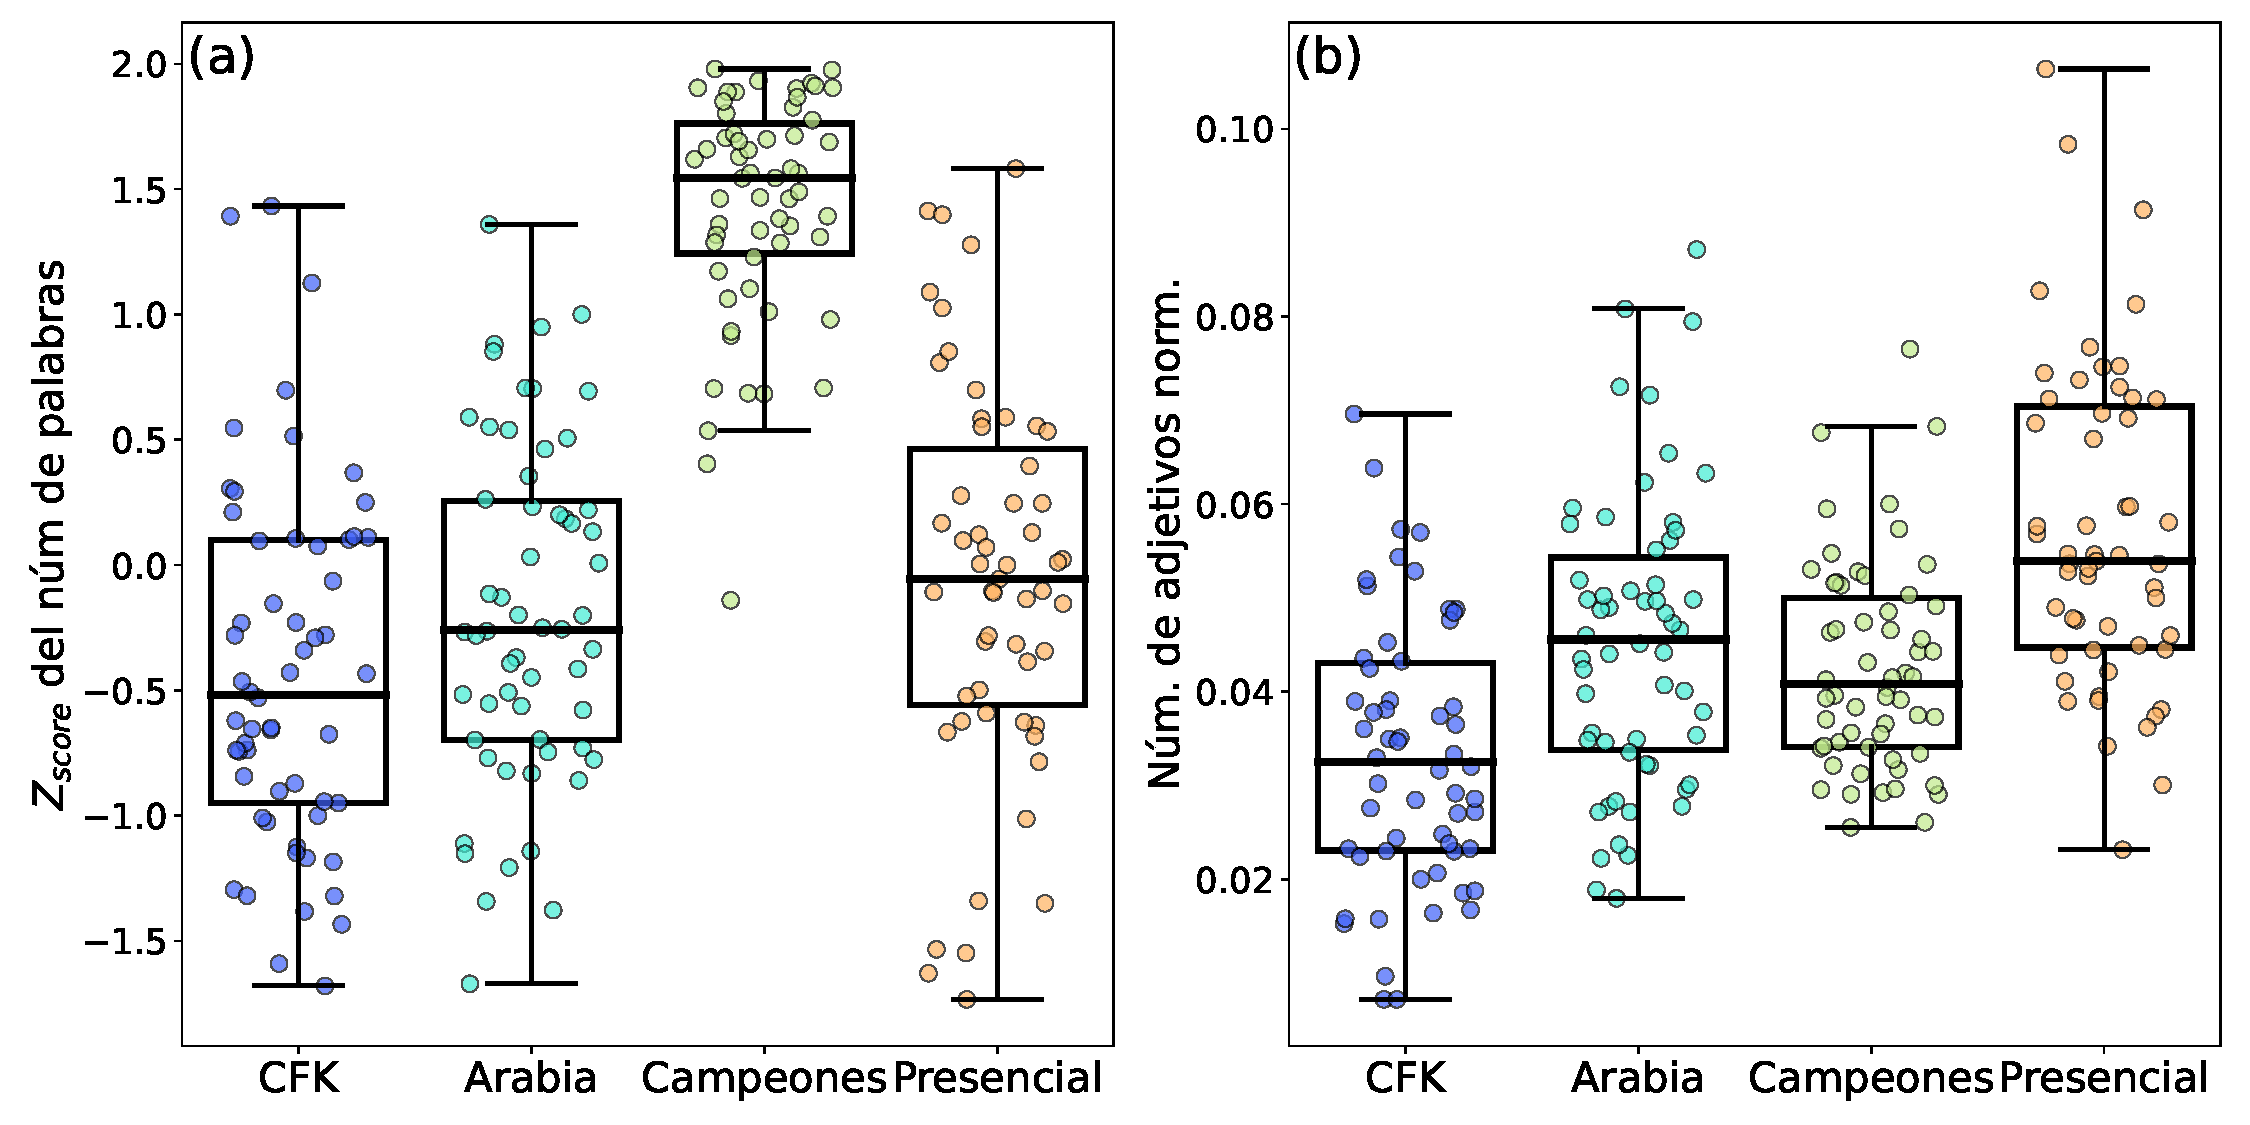
\includegraphics[width = 15cm]{figures/ch03/Herramientas NPL/Primer tiempo/Sin control/contenido_boxplot.pdf} 
    \caption{\textbf{(a)}  \textbf{(b)}}
\label{fig:cap3_vars_contenido}
\end{figure}

\begin{figure}[H]
    \centering
    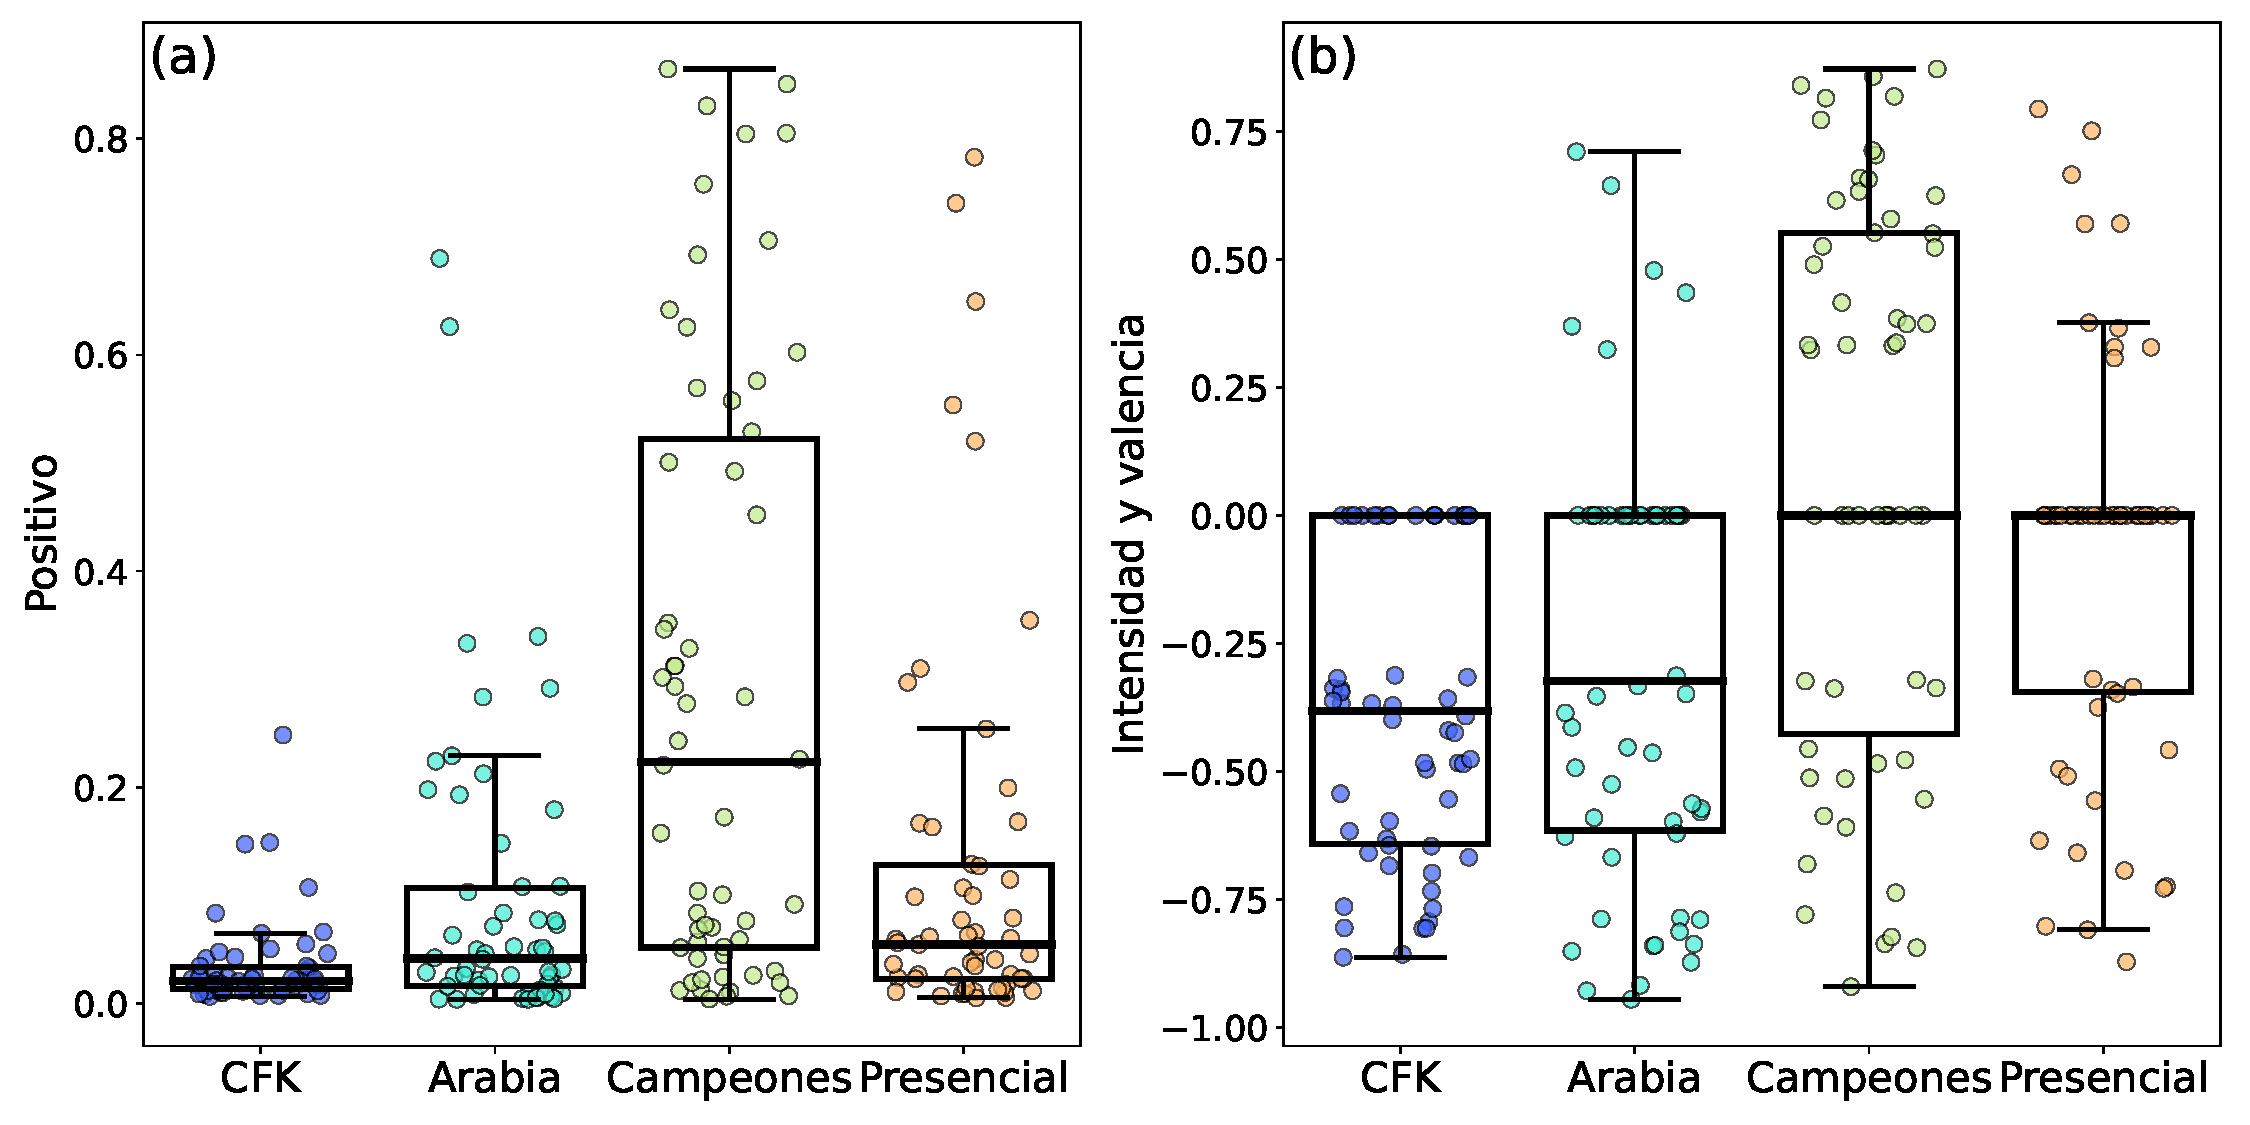
\includegraphics[width = 15cm]{figures/ch03/Herramientas NPL/Primer tiempo/Sin control/sentimiento_boxplot.pdf} 
    \caption{\textbf{(a)}  \textbf{(b)}}
\label{fig:cap3_vars_sentimiento}
\end{figure}

\begin{figure}[H]
    \centering
    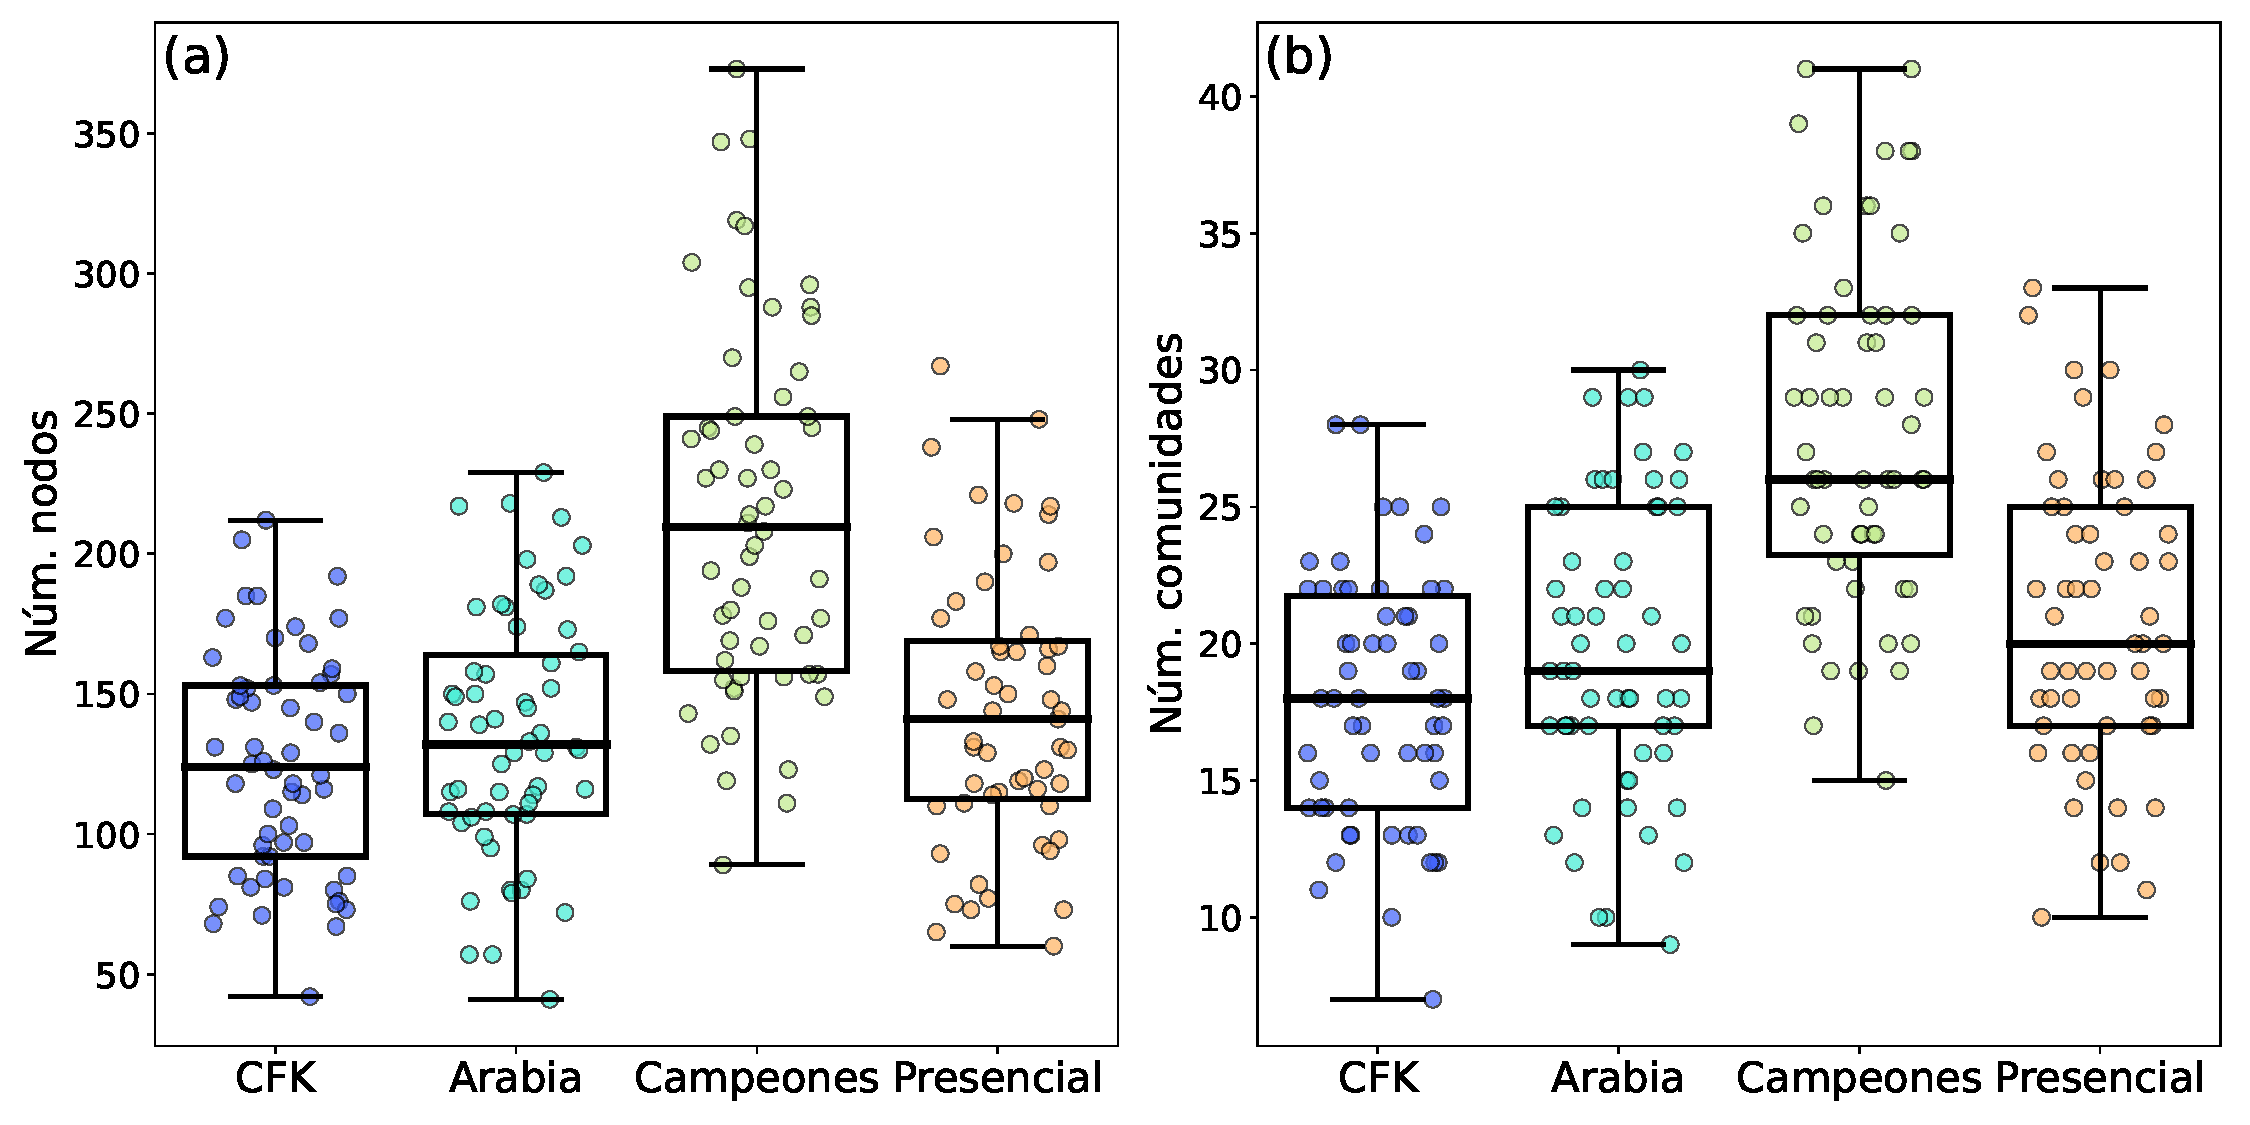
\includegraphics[width = 15cm]{figures/ch03/Herramientas NPL/Primer tiempo/Sin control/estructurales1_boxplot.pdf} 
    \caption{\textbf{(a)}  \textbf{(b)}}
\label{fig:cap3_vars_sentimiento}
\end{figure}


\begin{figure}[H]
    \centering
    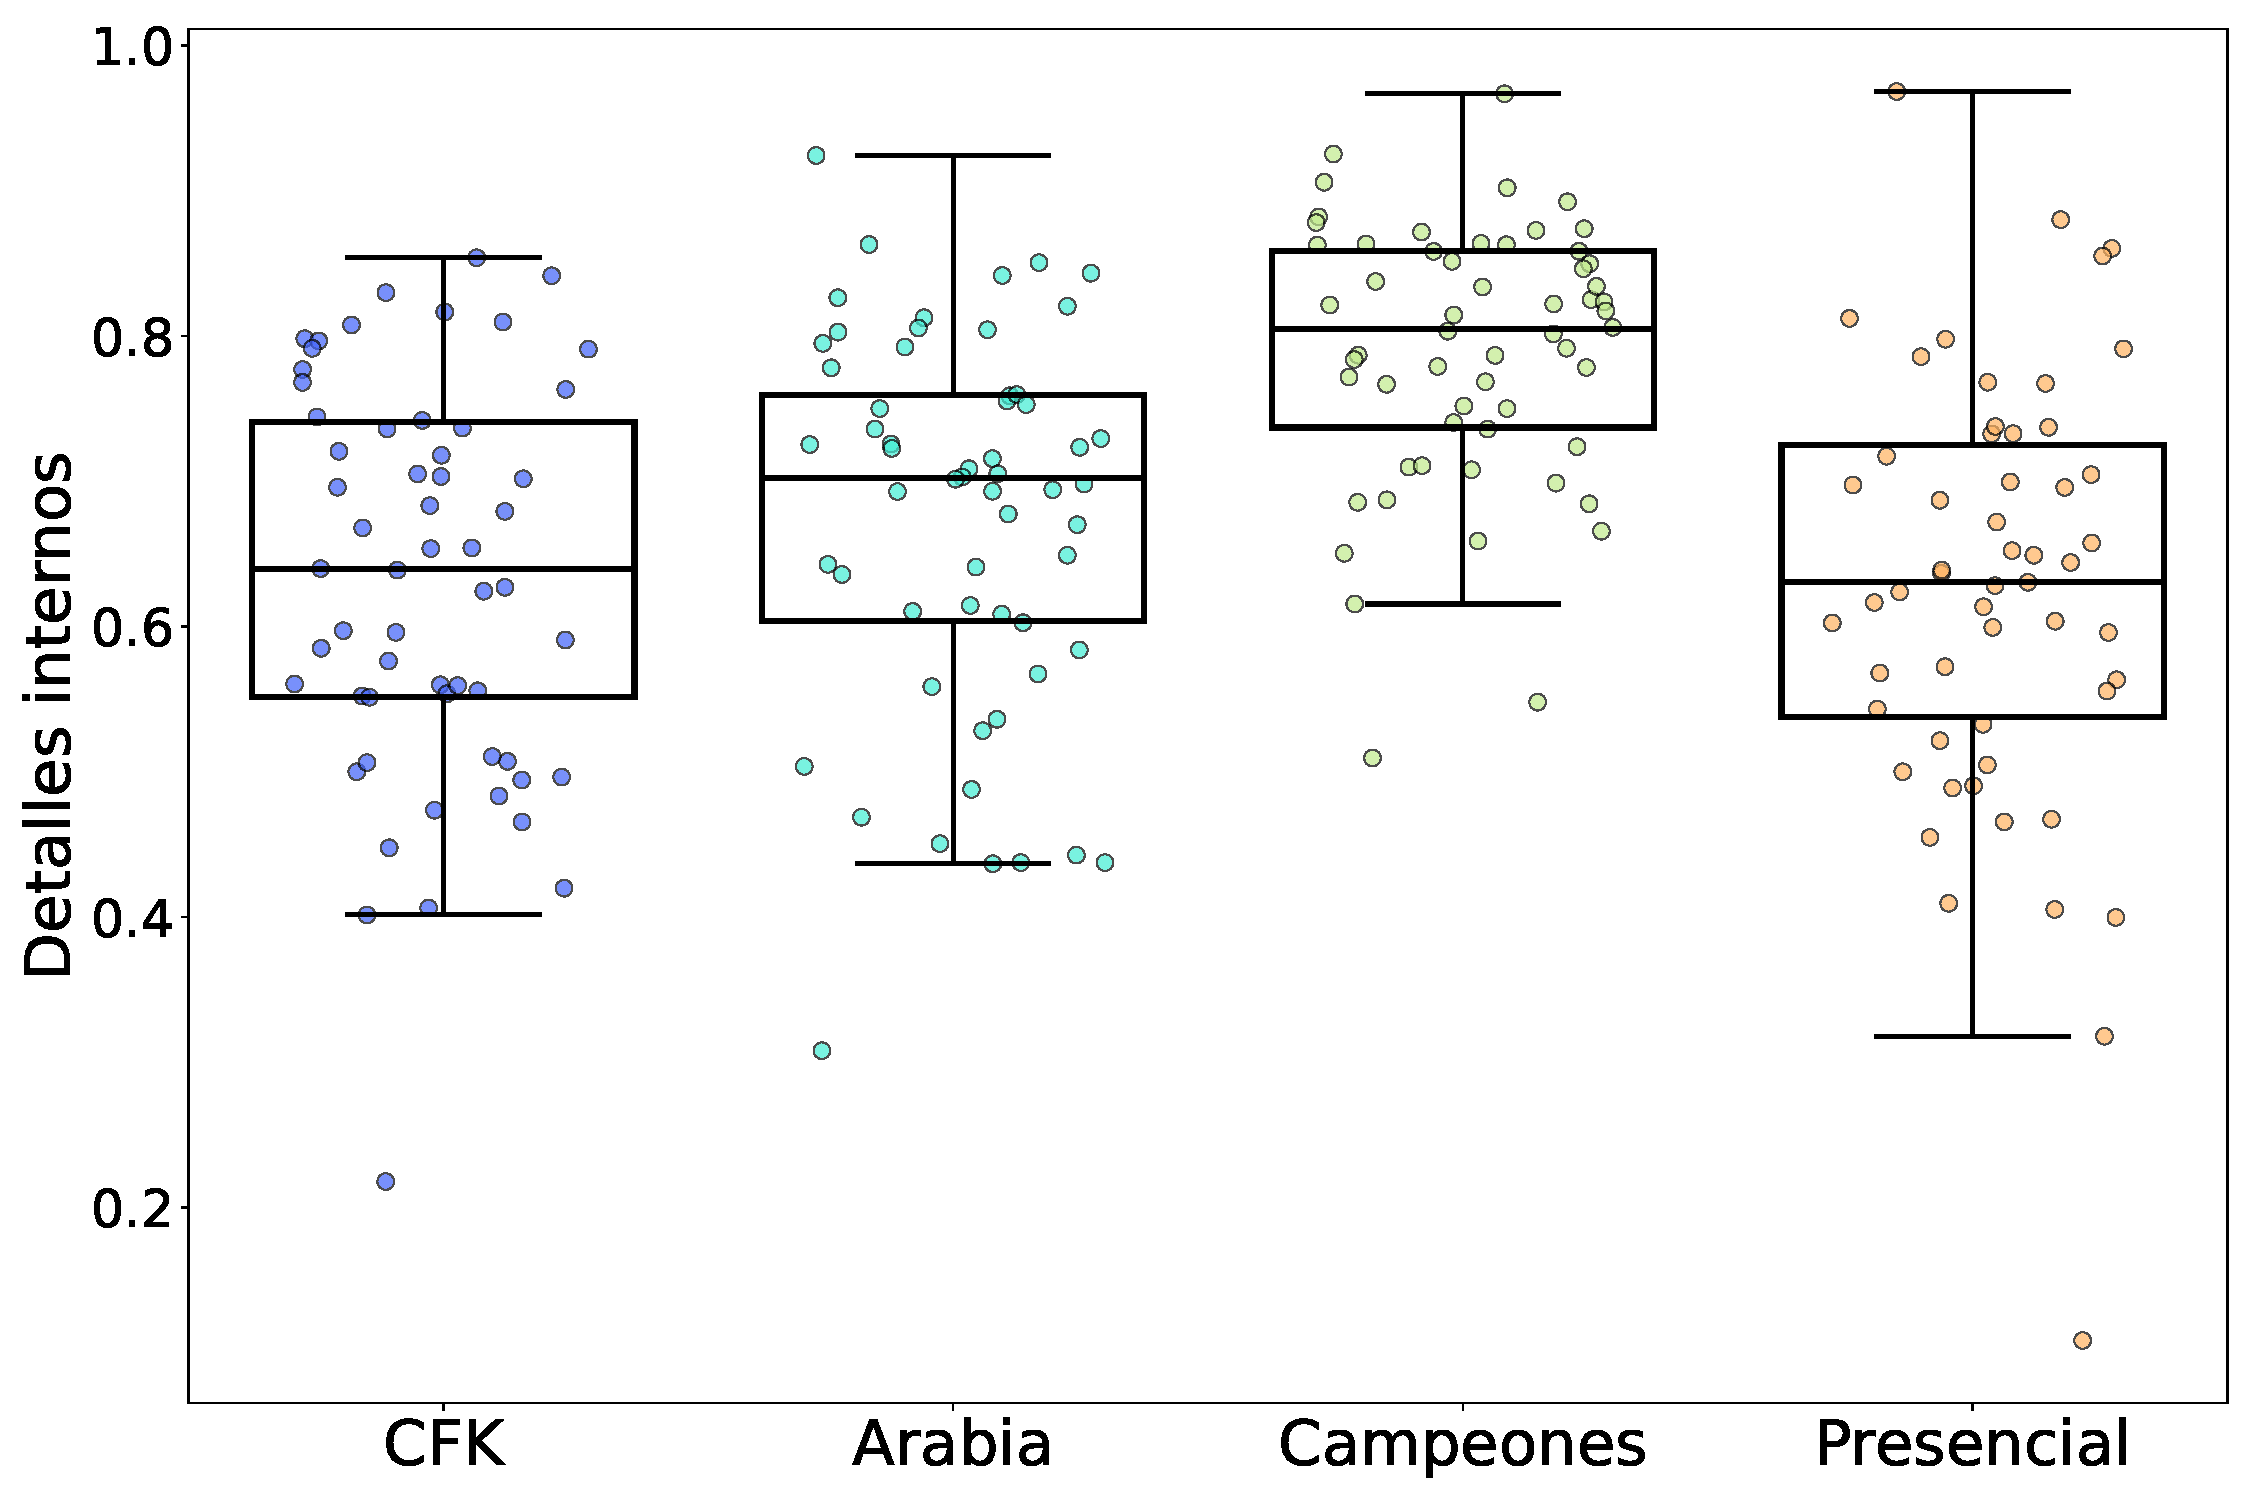
\includegraphics[width = 11cm]{figures/ch03/Herramientas NPL/Primer tiempo/Sin control/memoria_boxplot.pdf} 
    \caption{\textbf{(a)}  \textbf{(b)}}
\label{fig:cap3_var_memoria}
\end{figure}
\end{comment}
Para los cuantificadores de contenido se graficó para cada condición las variables del número de palabras únicas, número de adjetivos y número de pronombres en primera persona como se puede observar en la Figura \ref{fig:cap3_vars_contenido} (a), (b) y (c), respectivamente. Como se observa en la  Figura \ref{fig:cap3_vars_contenido} (a) los participantes hablaron en promedio en la condición campeones, el cual era el relato mas intenso en la validación externa. Luego en presencial hablaron como en su media, y en CFK y Arabia hablaron por debajo de su media. El análisis de ANOVA reportó que hay diferencias significativas entre las medias de los grupos (F$_{3, 138}$ = 61,45, p $<$ 3$\times$10$^{-25}$, $\eta_g^2$ = 0,56). El posterior análisis de Tuckey encontró que la diferencia significativa se da entre el grupo campeones con los demás, en todos los casos con p $<$ 9$\times$10$^{-15}$. \colorbox{yellow}{tengo que aclarar que usé oneway anova en métodos, pero cómo se dice oneway anova en español?, y no debería chequear que los datos sigan una distribución normal?} 
\colorbox{yellow}{aclarar en métodos que se tuvo en cuenta corrección al pval para pasar significancia de tuckey por repetir con varios grupos}
Para el número de adjetivos se observa en la Figura \ref{fig:cap3_vars_contenido}(b) el mayor uso en la condición presencial y el menor uso en la condición de CFK, se hallaron diferencias significativas entre las medias de los grupos (F$_{3, 138}$ = 20,16, p $<$ 7$\times$10$^{-11}$, $\eta_g^2$ = 0,22), en particular entre presencial y CFK con todos las demás condiciones y entre ellas (p $<$ 3$\times$10$^{-3}$). 
Para finalizar con las variables de contenido se graficó el número de palabras en primera persona en la Figura \ref{fig:cap3_vars_contenido}(c). Se puede observar que presencial por mas que es el único relato no colectivo \colorbox{yellow}{hablar de relatos colectivos en intro} es el que menor cantidad de pronombres de primera persona tiene. Del análisis de ANOVA se obtienen diferencias significativas entre las medias (F$_{3, 138}$ = 14,74, p $<$ 3$\times$10$^{-8}$, $\eta_g^2$ = 0,17). El posterior análisis de Tuckey dió que las diferecias son entre la condición presencial con las demás tres condiciones ( p $<$ 4$\times$10$^{-5}$).

\begin{figure}[H]
    \centering
    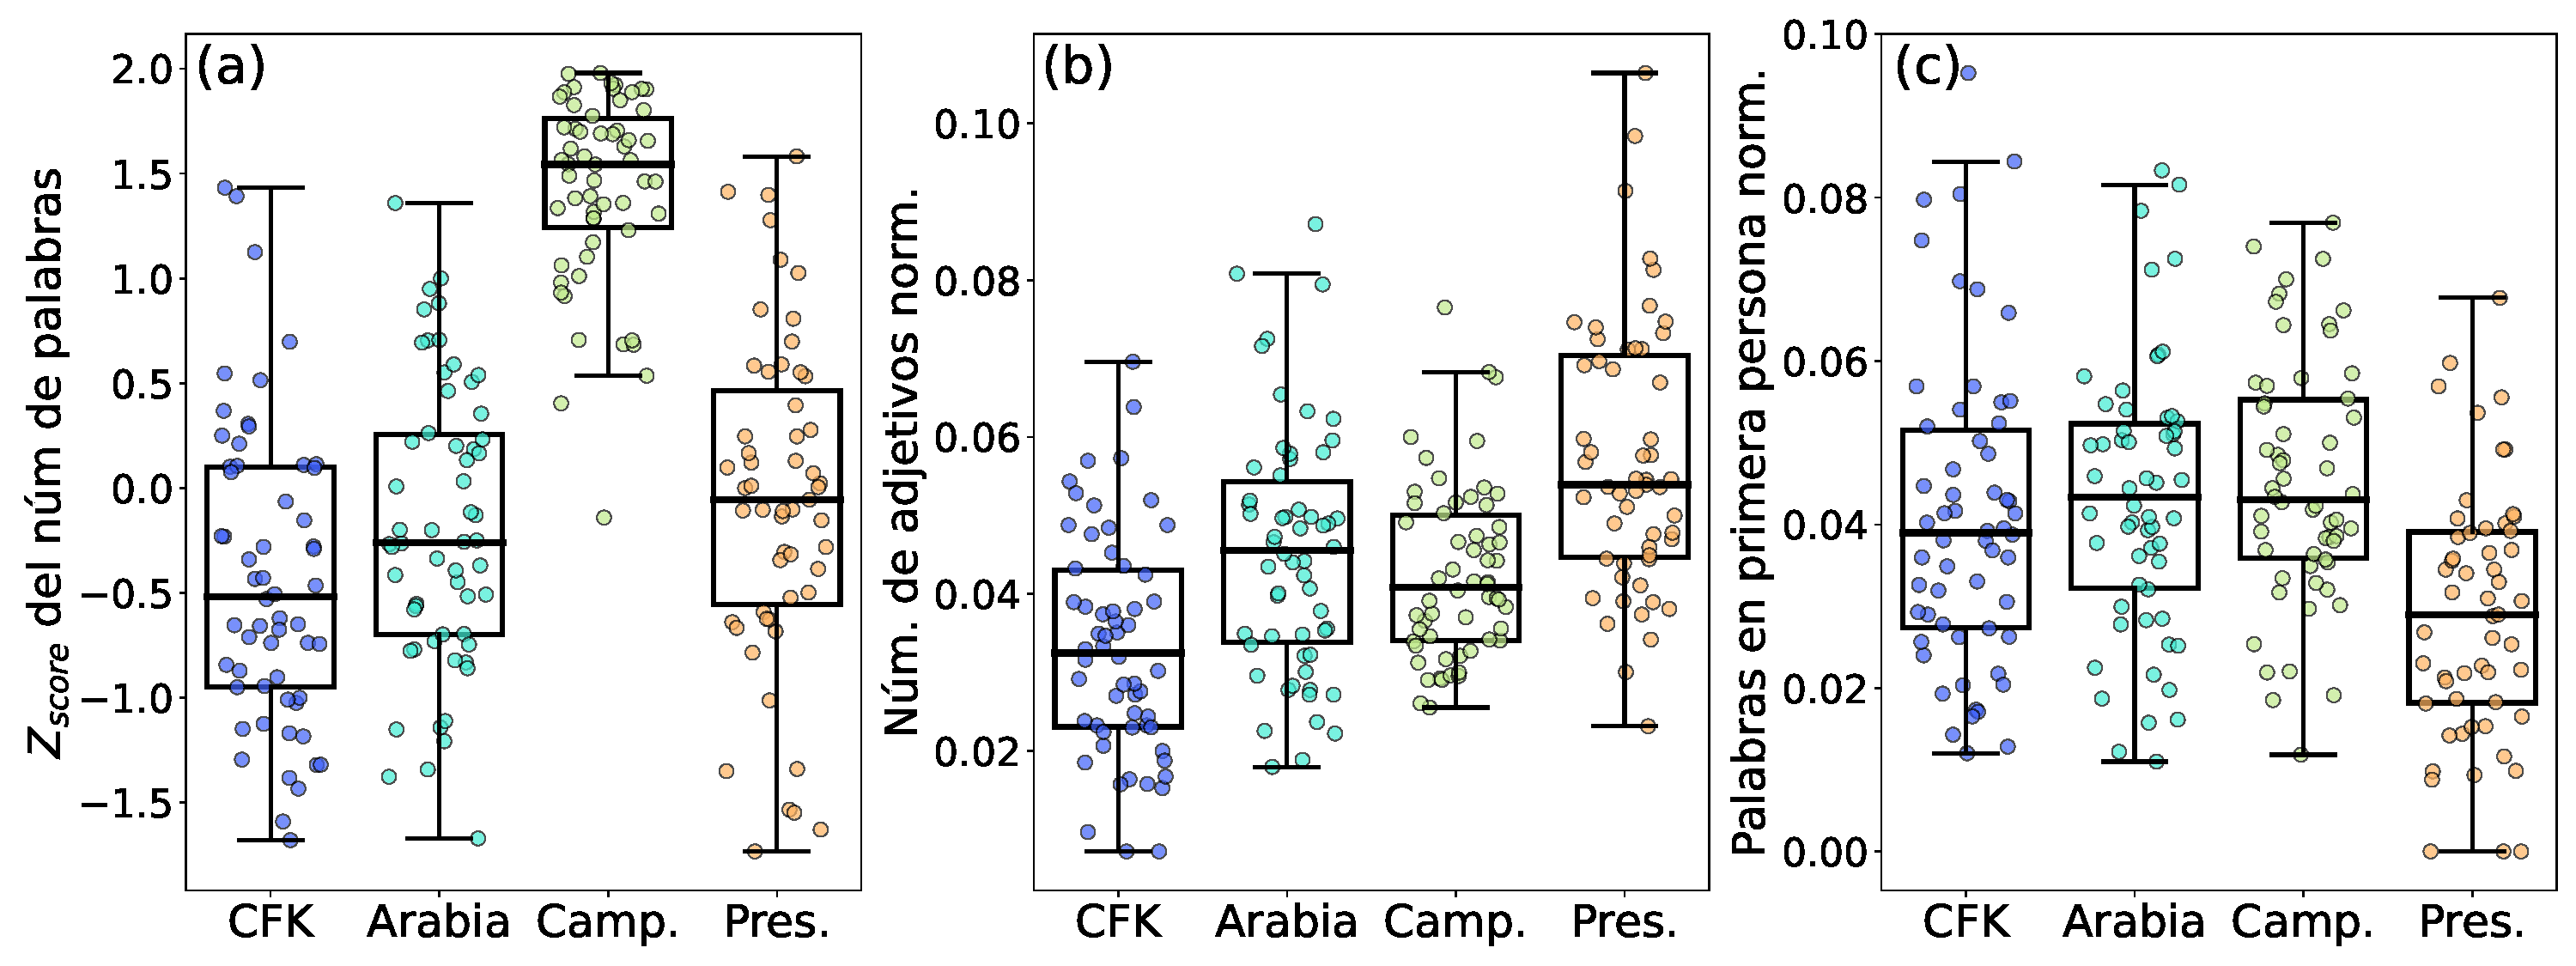
\includegraphics[width = 15cm]{figures/ch03/Herramientas NPL/Primer tiempo/Sin control/contenido_op2_boxplot.pdf} 
    \caption{Boxplots para las distintas condiciones para variables de contenido. En particular en \textbf{(a)} el número de palabras únicas normalizadas con el $Z_{score}$ con los relatos de un mismo sujeto en las diferentes condiciones,  \textbf{(b)} el número de adjetivos normalizado por el número de palabras totales del relato, \textbf{(c)} el número de palabras en primera persona normalizado por el número de palabras en el relato.}
\label{fig:cap3_vars_contenido}
\end{figure}

Continuando con los cuantificadores de sentimiento se graficó en la Figura \ref{fig:cap3_sent_barras} la probabilidad promedio (entre todos los sujetos) de que una condición sea positiva, negativa o intensa (la suma de las dos anteriores). Se puede observar que solo hay diferencias significativas en la intensidad para la condición de presencial respecto de las otras tres, siendo este el menos intenso de todos los relatos. En tanto a la probabilidad de que el relato sea negativo, no se obtuvo diferencia significativas entre las condiciones de CFK y Arabia, ni entre las condiciones de campeones con presencial. Se obtuvo que el primer par son las condiciones mas negativas. Por último la probabilidad de que el relato sea positivo solo no dio diferencias significativas entre las condiciones de Arabia y presencial. Se obtuvo que el relato mas positivo es campeones y el menos positivo es CFK.

\begin{figure}[H]
    \centering
    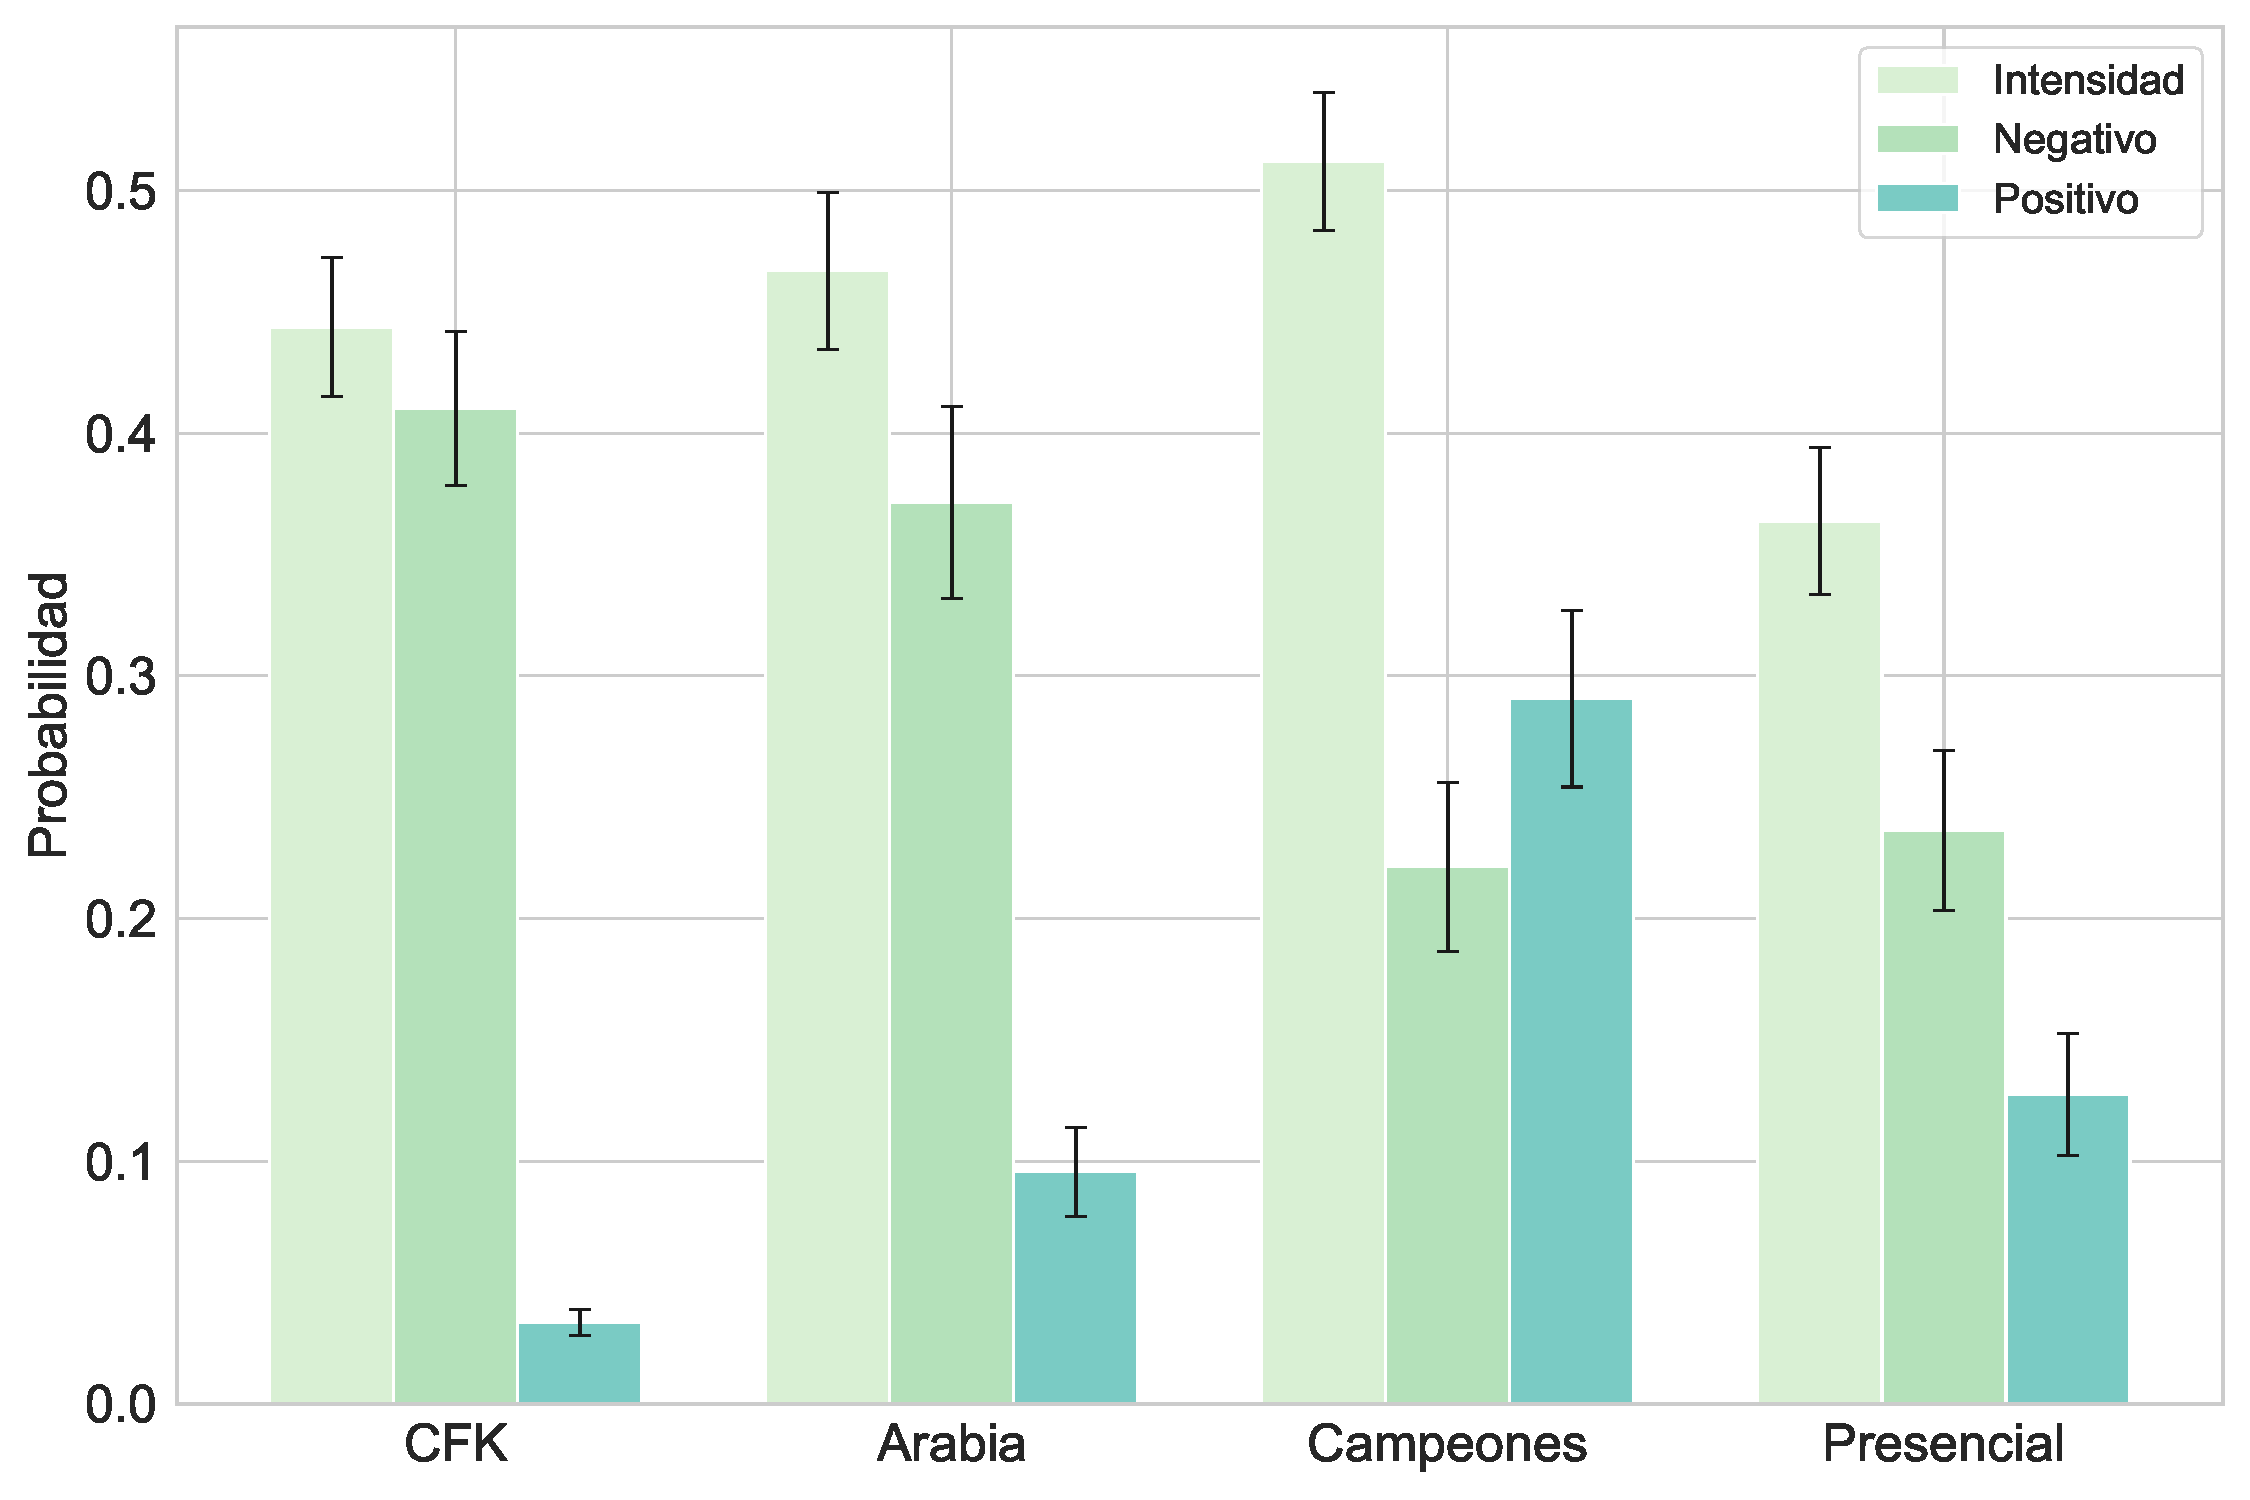
\includegraphics[width = 15cm]{figures/ch03/Herramientas NPL/Primer tiempo/Sin control/pysentimiento_tresbarras.pdf} 
    \caption{Gráfico de la probabilidad de promedio (entre sujetos) de que las condiciones sean positivas negativas o intensas (la suma de las últimas dos) dado de las herramientas de NPL. Estos cuantificadores fueron obtenidos como se indica en \colorbox{yellow}{citar métodos donde explique esto}.}
\label{fig:cap3_sent_barras}
\end{figure}

Luego se realizaron boxplots para algunas de los cuantificadores de sentimiento, los mismos se pueden observar en la Figura \ref{fig:cap3_vars_sentimiento}. En particular, en la Figura \ref{fig:cap3_vars_sentimiento}(a) se observa la variable que denota la probabilidad de que un realto sea positivo. Al igual que se observaba en la Figura \ref{fig:cap3_sent_barras} se tiene que condición mas positiva es campeones y la menos positiva CFK. Existen diferencias significativas entre las medias de los grupos (F$_{3, 138}$ = 16,55, p $<$ 9$\times$10$^{-7}$, $\eta_g^2$ = 0,21) en particular entre campeones y CFK con las otras dos condiciones y entre ellas ( p $<$ 3$\times$10$^{-3}$).

Luego en la Figura \ref{fig:cap3_vars_sentimiento}(b) se observa los boxplots de la variable de intensidad y valencia para las cuatro condiciones. En la misma se puede observar una alta probabilidad densidad de puntos en el cero que denota los relatos que tenian mayor probabilidad de ser neutros. Luego se puede ver que campeones es la condición con mayor cantidad de relatos positivos, sin embargo su mediana al igual que la de presencial es nula. Para los relatos de CFK y Arabia se obtienen medianas negativas. El análisis de ANOVA dió que hay diferencias significativas entre las medias (F$_{3, 138}$ = 10,11, p $<$ 5$\times$10$^{-6}$, $\eta_g^2$ = 0,14) y el posterior analisis de Tuckey reveló que las mismas son entre la condición campeones con CFK y Arabia ( p $<$ 0,0014) y entre CFK y presencial (p $<$ 0,0006).

El último cuantificador de sentimiento graficado es la intensidad y se observa en la Figura \ref{fig:cap3_vars_sentimiento}(c), al igual que como se obserba en la Figura \ref{fig:cap3_sent_barras} la condición menos intensa resulta ser presencial. El análisis de ANOVA muestra diferencia significativa entre las medias (F$_{3, 138}$ = 3,64, p $<$ 0,01, $\eta_g^2$ = 0,05), la prueba de Tuckey muestra que la diferencia significativa se da entre las condiciones campeones y presencial (p $<$ 0.0035).

\begin{figure}[H]
    \centering
    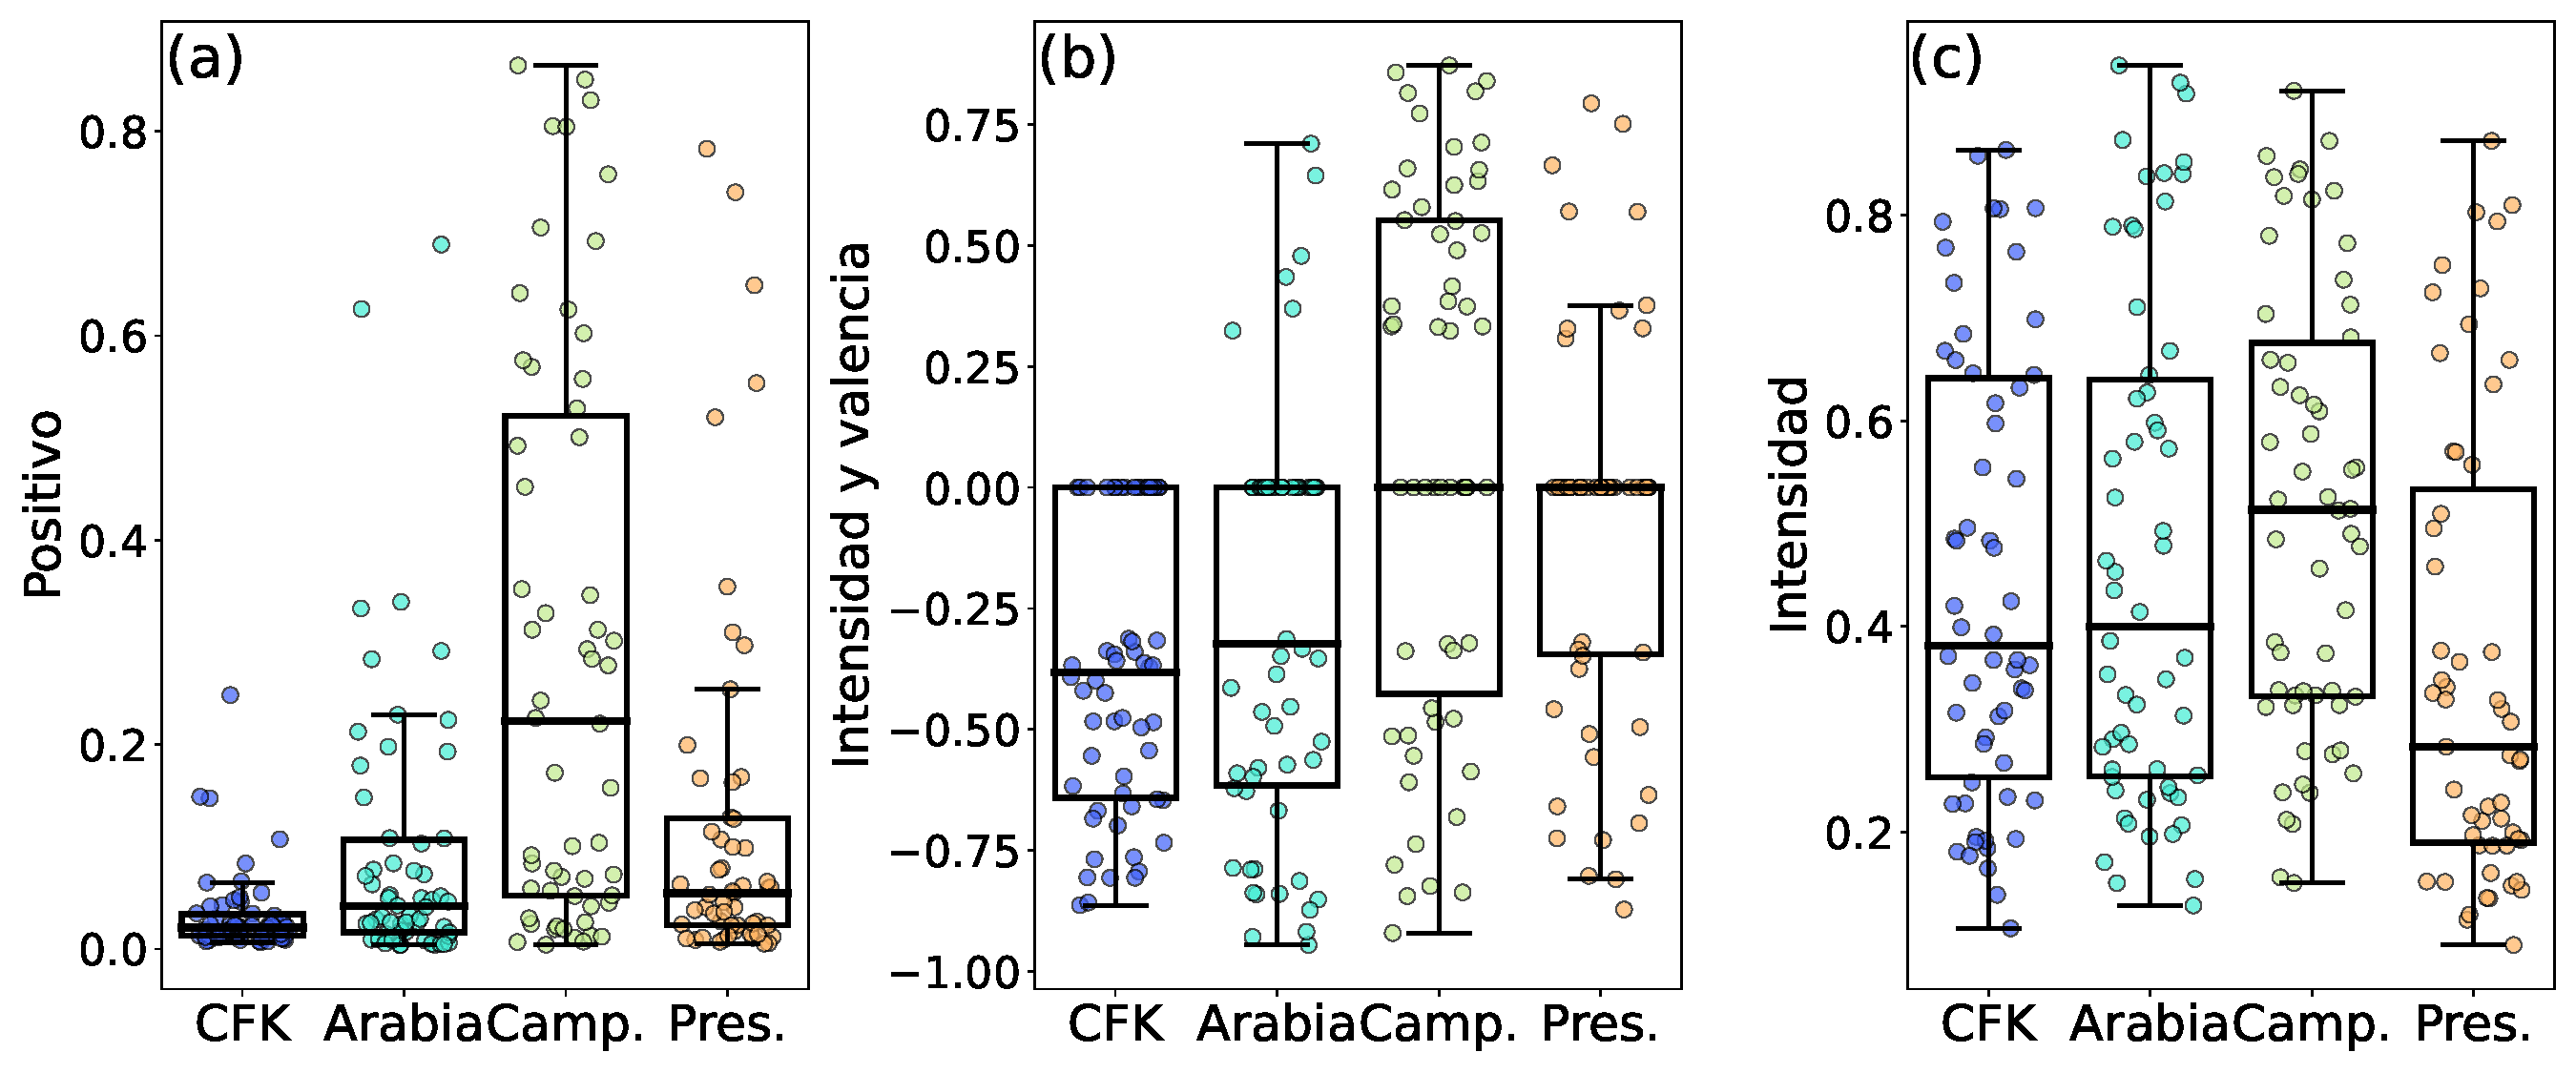
\includegraphics[width = 15cm]{figures/ch03/Herramientas NPL/Primer tiempo/Sin control/sentimiento_op2_boxplot.pdf} 
    \caption{Boxplots para las distintas condiciones para variables de sentimiento. En particular en \textbf{(a)} la probabilidad de que el relato sea positivo. En \textbf{(b)} la valencia por la intensidad. En \textbf{(c)} la intensidad del relato (suma de la probabilidad de negativo mas positivo).}
\label{fig:cap3_vars_sentimiento}
\end{figure}

Continuando con las variables estructurales, inicialmente se observó si la coherencia disminuye con la distancia entre las oraciones al calcularla. Se construyó un modelo nulo promedio como se explicó en \colorbox{yellow}{citar} y se calculó la coherencia promedio entre los sujetos para cada condición. Esto es lo que se puede observar graficado en la Figura \ref{fig:cap3_coherencia_d}, donde la línea punteada negra denota el modelo nulo promedio. Se observa que la coherencia efectivamente disminuye al aumentar la distancia entre oraciones y además se ve un comportamiento sostenido en la distancia donde la coherencia media de la condición Arabia es la mayor y la de presencial la menor. \colorbox{yellow}{Esto podría deberse al hecho de que presencial es el mas lejano en el tiempo, asi como también el menos intenso.}


\begin{figure}[H]
    \centering
    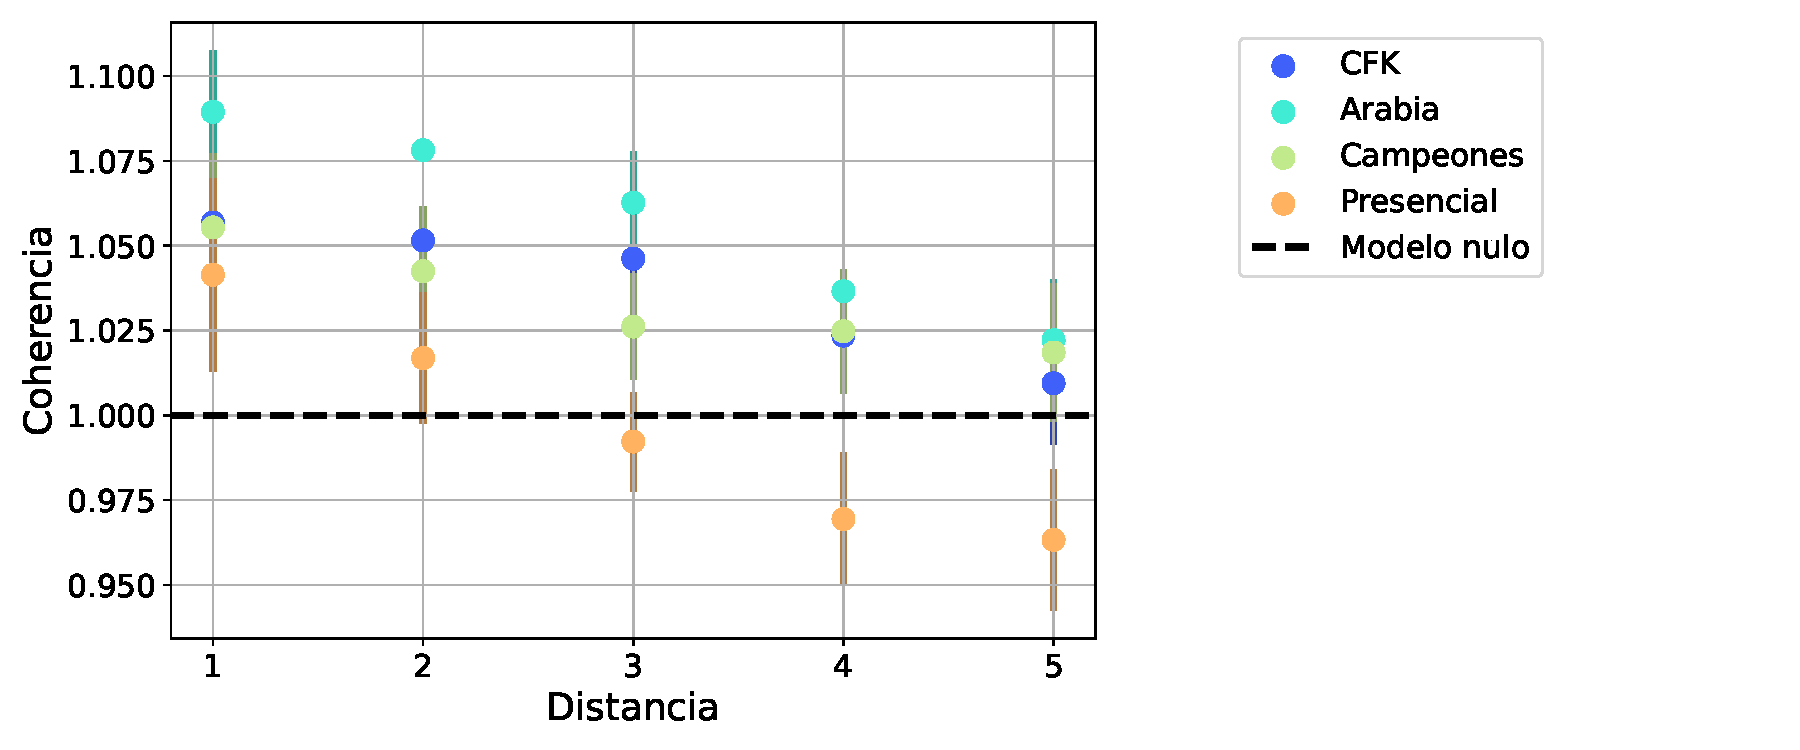
\includegraphics[width = 15cm]{figures/ch03/Herramientas NPL/Primer tiempo/Sin control/coherencia_vs_t_conmodelonulo.pdf} 
    \caption{Coherencia promedio (entre los sujetos) para cada condición en función de la distancia entre las oraciones utilizada para calcularla. La linea negra punteada denota el modelo nulo promedio.}
\label{fig:cap3_coherencia_d}
\end{figure}

En la Figura \ref{fig:cap3_vars_estructurales} (a), (b) y (c) se pueden observar tres cuantificadores estructurales. En (a) la coherencia utilizando una distancia de 3 (es decir, calculando la coherencia del relato entre oraciones que se encuentran separadas por tres de ellas). En (b) el número de nodos de la componente fuertemente conexa del grafo hecho a partir del relato, y en (c) el número de comunidades de la misma componente. En la Figura \ref{fig:cap3_vars_estructurales}(a) se puede observar como la coherencia a distancia 3 es similar en todas las condiciones lo cual es confirmado con el análisis de ANOVA con el cual no se obtiene diferencia significativa entre las medias (p = 0,08). Resultados similares se obtienen para distancia 1 y 2. En tanto a las variables que son atributos de la red de grafo armada del relato de los participantes se tiene en todas un F significativo, en particular en en el número de nodos y comunidades en la componente fuertemente conexa como se ve en la Figura \ref{fig:cap3_vars_estructurales}(b) y (c) la condición de campeones tiene una mediana mayor a las demás condiciones, el ANOVA de cada caso es respectivamente F$_{3, 138}$ = 50,18, p $<$ 5,5$\times$10$^{-22}$, $\eta_g^2$ = 0,38 y F$_{3, 138}$ = 42,38,  p $<$ 1,8$\times$10$^{-19}$, $\eta_g^2$ = 0,37. El análisis de Tuckey muestra que en ambos casos la diferencia de la media es de campeones con las otras tres condiciones, en todos los casos con  p $<$ 7,8$\times$10$^{-10}$.
Sin embargo, este no es el comportamiento de todos los atributos de las redes de los relatos, se puede observar en la Figura \ref{fig:cap3_vars_mem}(a) la densidad que tiene un comportamiento contrario donde la condición de campeones tiene menor densidad que las demás (F$_{3, 138}$ = 23,79, p $<$ 1,8$\times$10$^{-12}$, $\eta_g^2$ = 0,27, Tuckey significativo entre campeones y las demás con p $<$ 3,2$\times$10$^{-9}$). O como para el coeficiente de clustering promedio que se observa en la Figura \ref{fig:cap3_vars_mem}(b) y se puede apreciar una menor diferencia entre las medias (F$_{3, 138}$ = 4,6, p $<$ 0,0043, $\eta_g^2$ = 0,06, Tuckey significativo entre campeones y presencial con p = 0,001).


\begin{figure}[H]
    \centering
    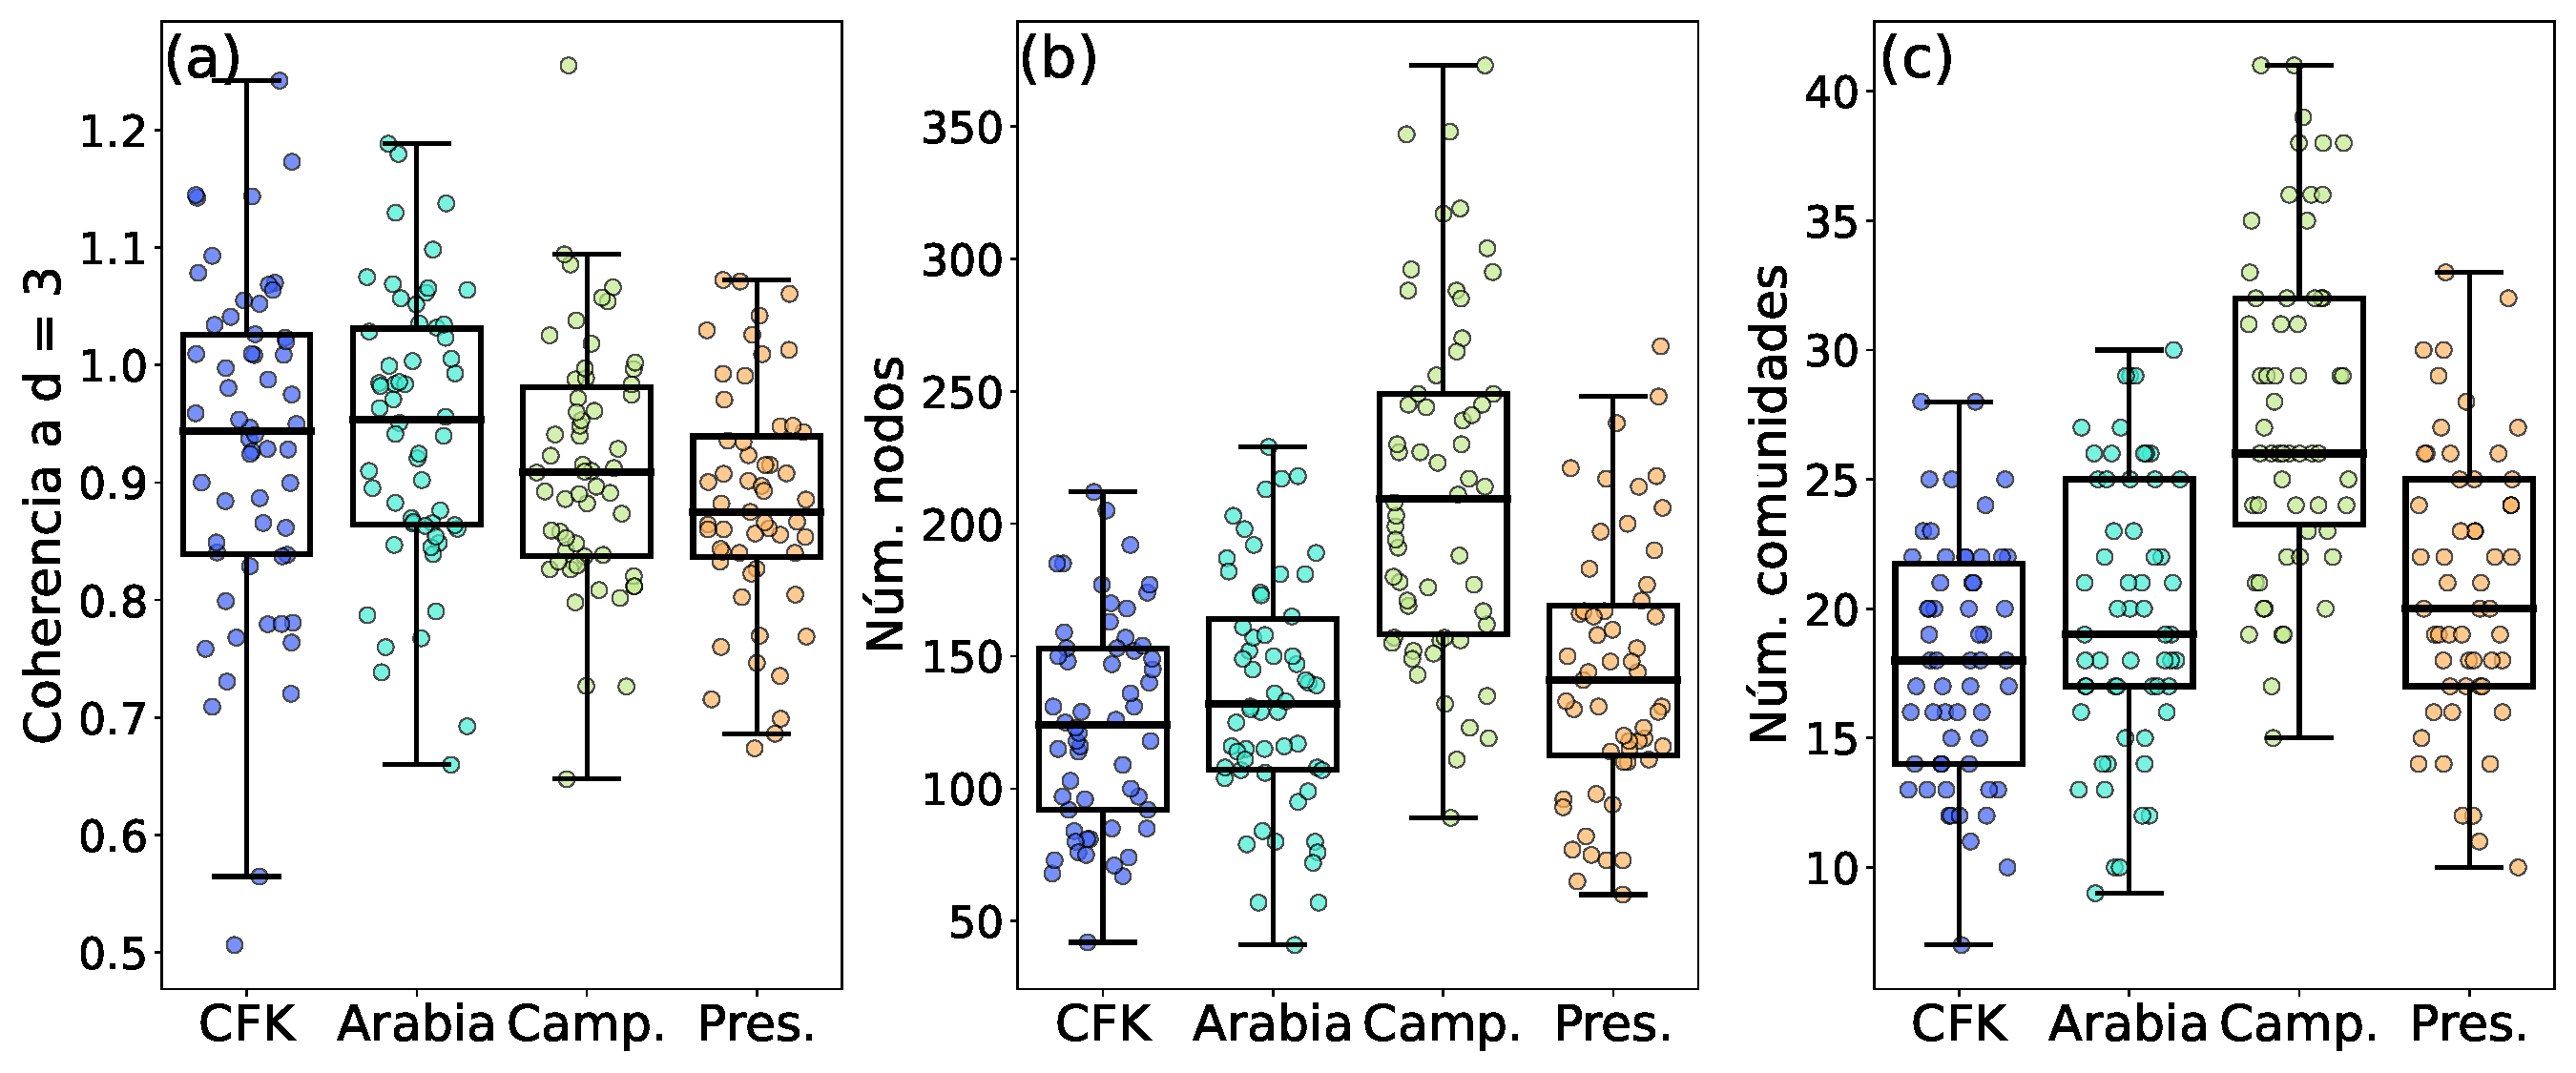
\includegraphics[width = 15cm]{figures/ch03/Herramientas NPL/Primer tiempo/Sin control/estructurales1op2_boxplot.pdf} 
    \caption{Gráfico de boxplot de diferentes variables estructurales para las distintas condiciones. En particular en \textbf{(a)} de la coherencia a distancia 3, en  \textbf{(b)} del número de nodos en la componente fuertemente conexa y en \textbf{(c)} del número de comunidades en la misma componente.}
\label{fig:cap3_vars_estructurales}
\end{figure}

Por último los cuantificadores de memoria que son detalles interno y externos. Como están anticorrelacionados vamos a solo observar el primero en la Figura \ref{fig:cap3_vars_mem}(c). Se puede observar una mayor cantidad de detalles internos en la condición de campeones y la menor en presencial. El ANOVA dio diferencia significativa entre las medias F$_{3, 138}$ = 21,3, p $<$ 2,2$\times$10$^{-11}$, $\eta_g^2$ = 0,22 y Tuckey significativo entre campeones y las demás condiciones con p $<$ 5$\times$10$^{-6}$.


\begin{figure}[H]
    \centering
    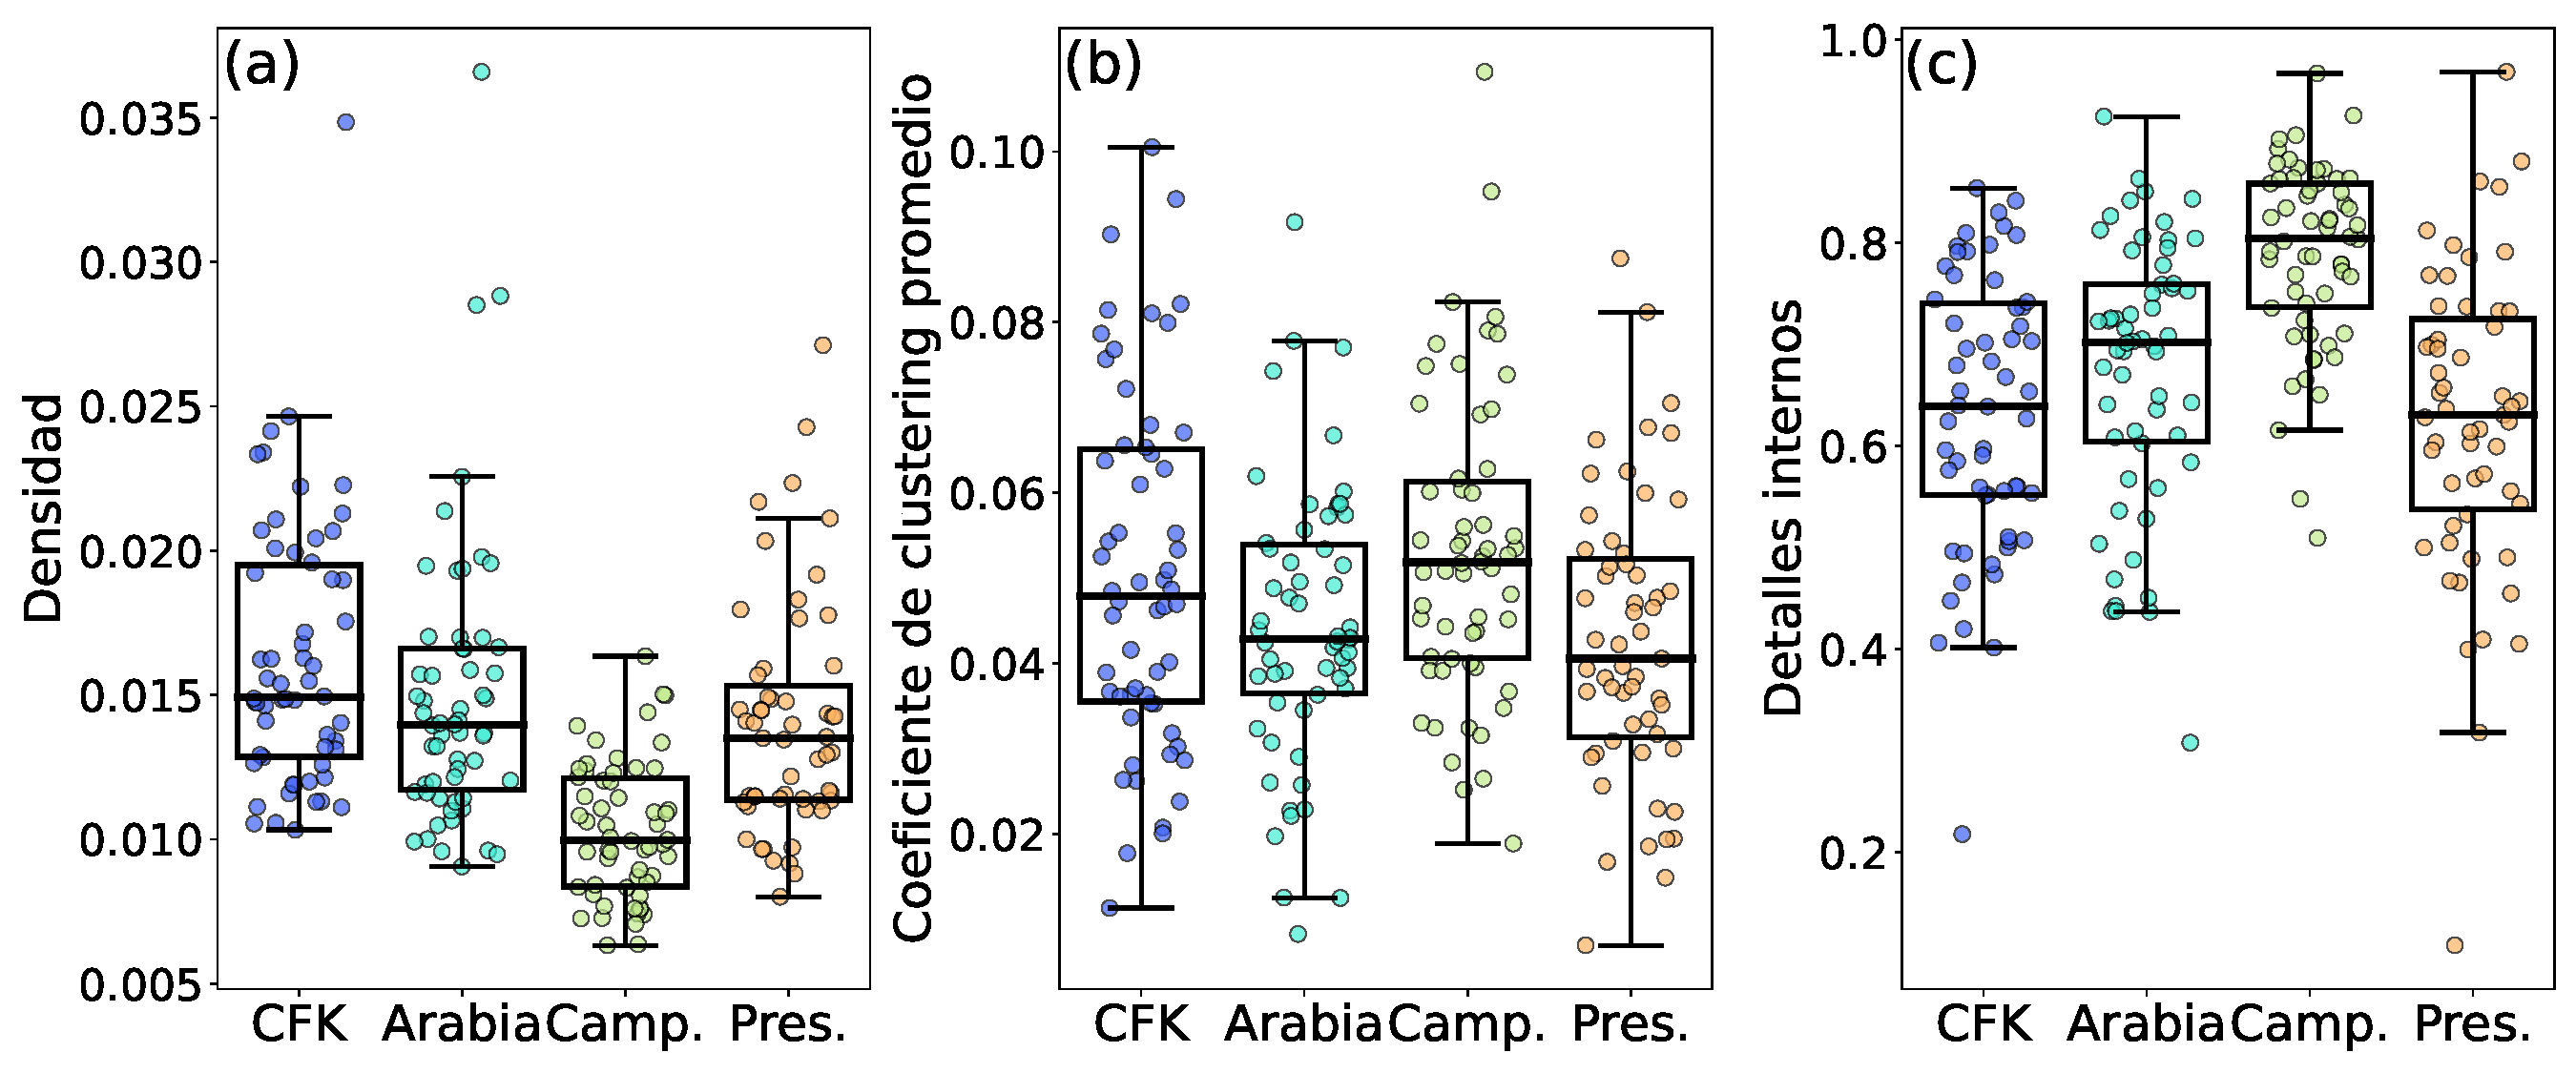
\includegraphics[width = 15cm]{figures/ch03/Herramientas NPL/Primer tiempo/Sin control/estructurales2op2_boxplot.pdf} 
    \caption{Boxplots para las distintas condiciones de variables estructurales y de memoria. En particular en \textbf{(a)} para la densidad de la red armada con los relatos, en \textbf{(b)} del coeficiente de clustering promedio de dicha red y en \textbf{(c)} la variable de memoria de detalles internos.}
\label{fig:cap3_vars_mem}
\end{figure}


\section{Correlación entre las variables del relato y de autopercepción}

Se estudió la correlación entre las variables discursivas incluyendo además las variables obtenidas de las respuestas del cuestionario posterior a la entrevista. Se obtuvo el resultado de la Figura \ref{fig:cap3_corr} para el primer tiempo, donde se grafica la matriz de correlación. El color blanco representa que el p$_{val}$ no fue significativo. Se tuvo en cuenta la corrección por las múltiples comparaciones (¿comparaciones? ¿cálculos?). 


\begin{figure}[h]
    \centering
    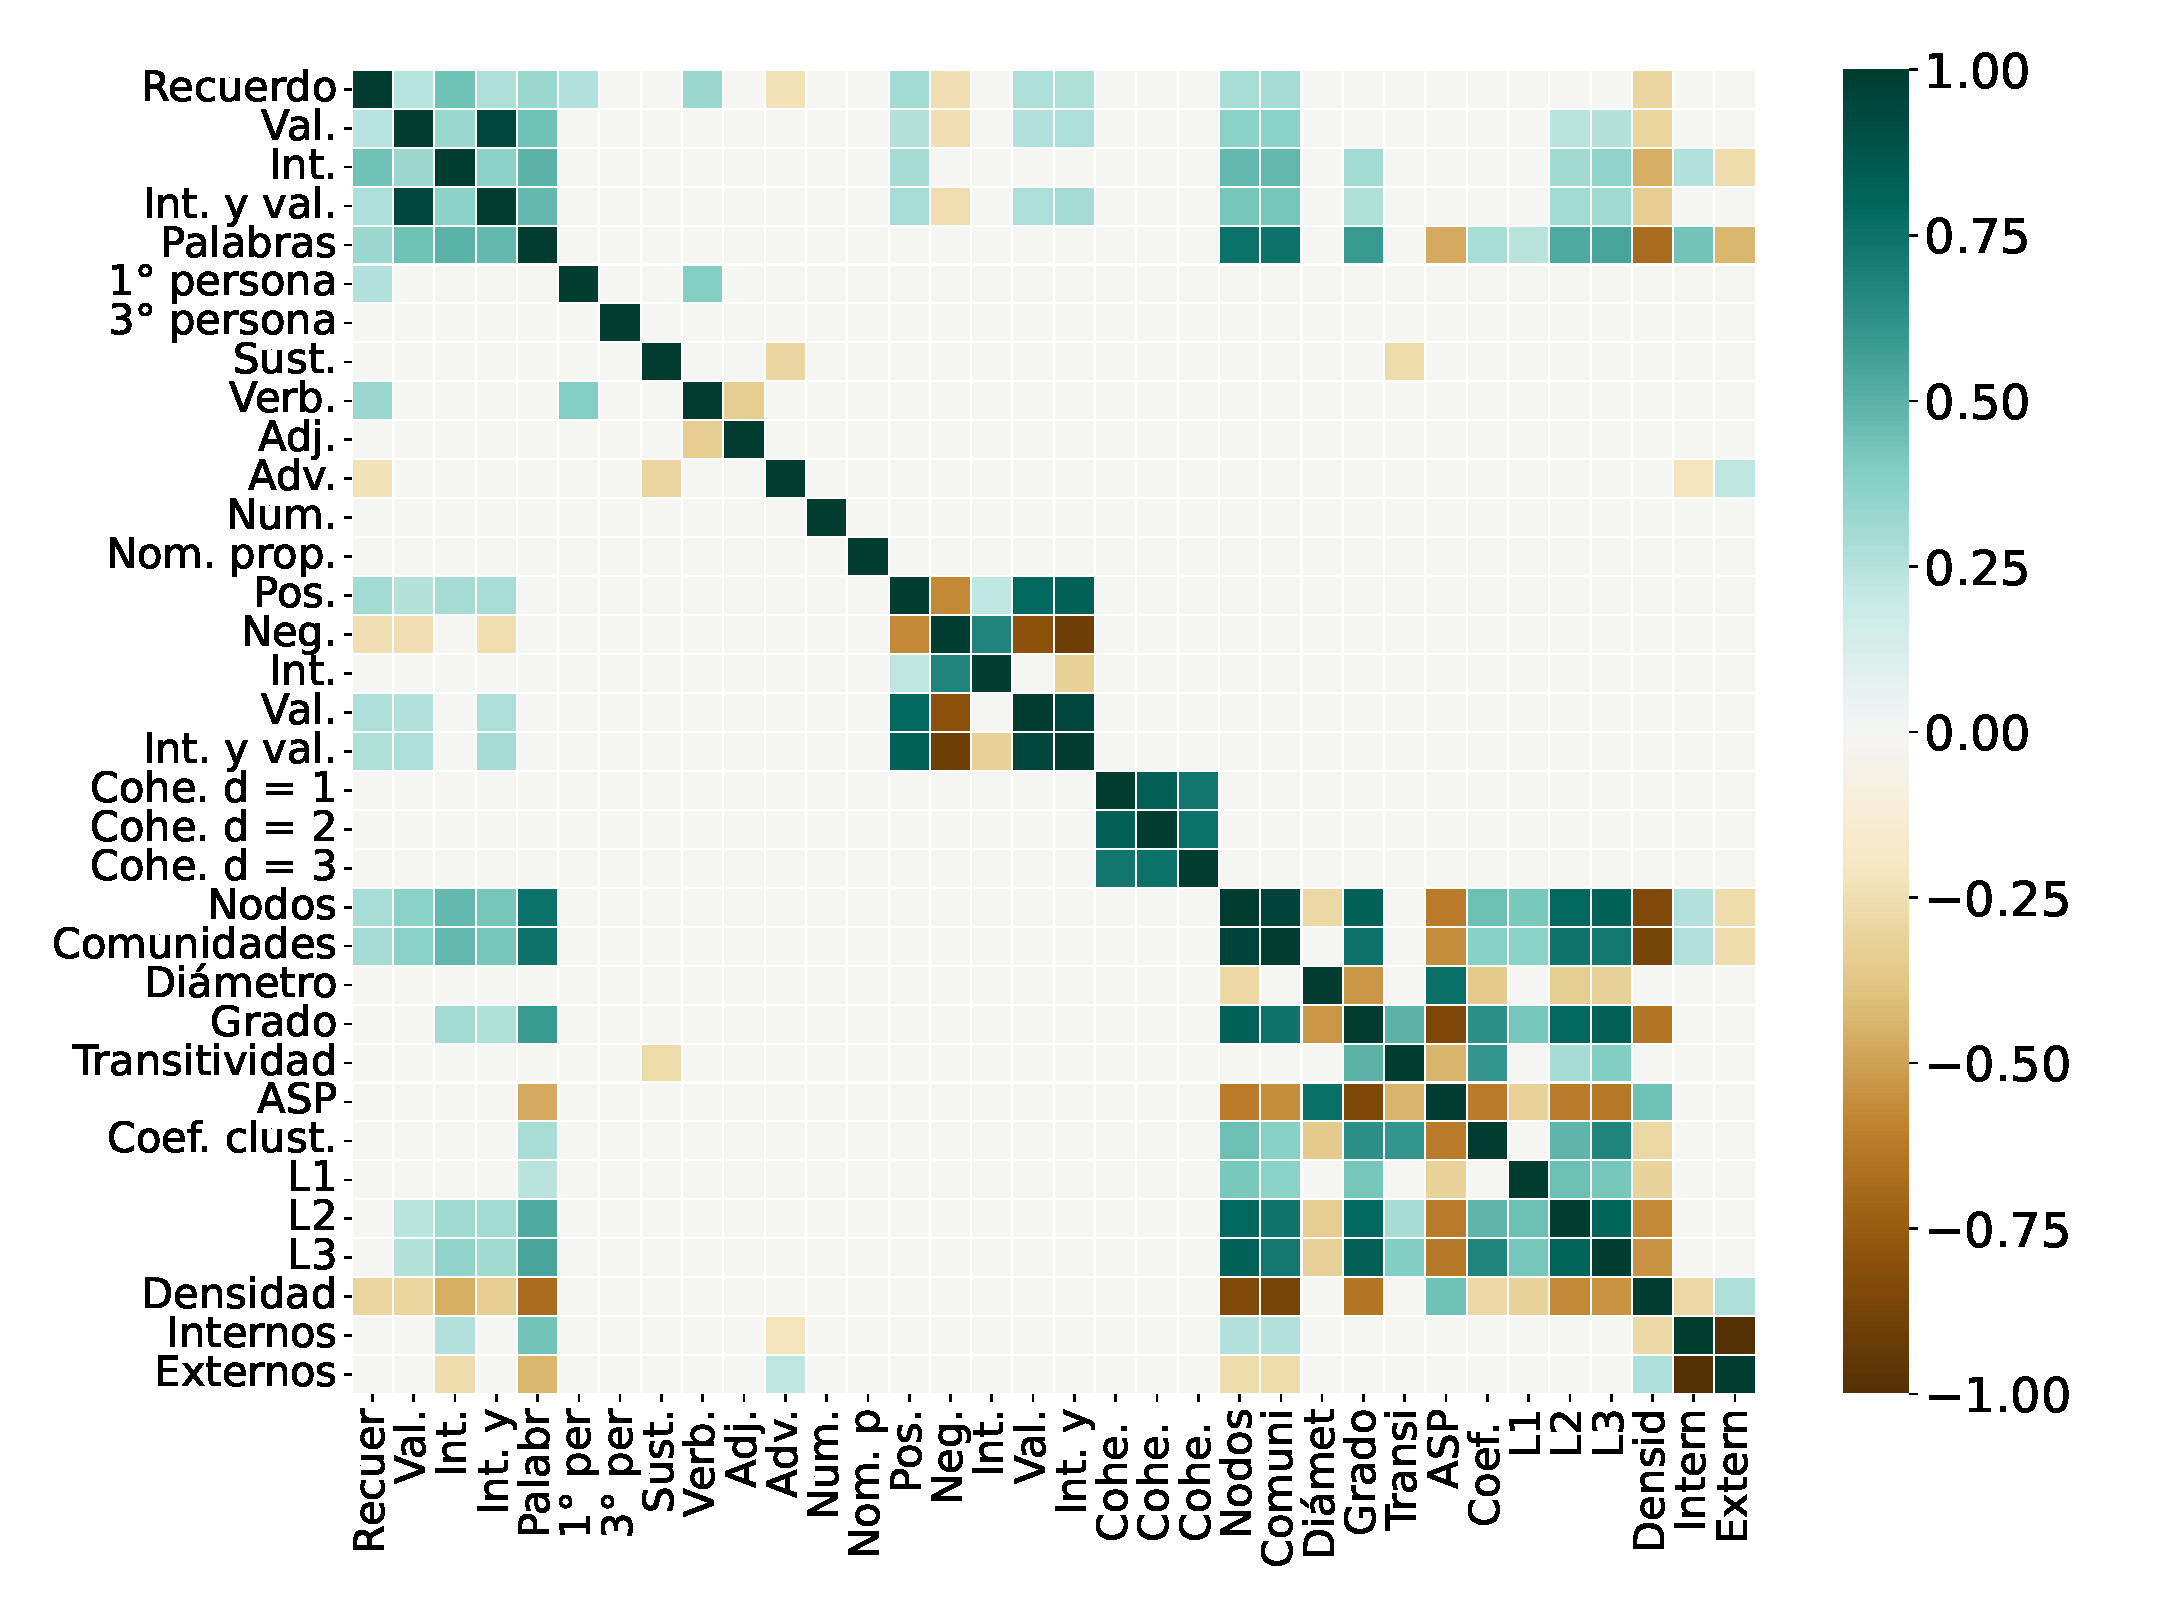
\includegraphics[width = 15cm]{figures/ch03/Correlacion/2correlacion_Primera.pdf} 
    \caption{Matriz de correlación de los cuantificadores de los relatos y las variables de autopercepción para la primer entrevista. Solo se presentan en color las correlaciones con un p$_{val}$ menor al significativo (9 $\times$ 10$^{-5}$ = 0,05/número de variables).}
\label{fig:cap3_corr}
\end{figure}

Se puede observar correlación entre todas las variables de autopercepción, y estas además correlacionan con el número de palabras. Es decir, cuando el número de palabras aumenta también lo hace el recuerdo valencia e intensidad autopercibida. Destaca además la correlación entre la valencia autopercibida con la calculada a través de pysentimiento y esto también sucede con la variable de intensidad y valencia. Con la variable de intensidad no se tuvo correlación.
El recuerdo autopercibido correlaciona con la variable positivo de pysentimiento, la valencia e intensidad y valencia, y anticorrelaciona con negativo. Es decir, los participantes dicen recordar mas los relatos clasificados como positivos y mas intensos, y menos los negativos y menos intensos. 
Además algunas variables de autopercepción correlacionan con algunas estructurales. Todas correlacionan con el número de nodos y comunidades en la componente fuertemente conexa que nos habla del largo del relato. Y también todas anticorrelacionan con la densidad, ... no se que decir de esto. Tampoco se que decir de las correlaciones con el grado y L2 Y L3...
Por último la intensidad autopercibida correlacionó con el número de detalles internos (episódicos) y anticorrelacionó con los externos (semánticos) lo cual es consistente con investigaciones previas (¿pongo citas en resultados?).
También correlaciona el recuerdo con primera persona verb y anticorr con adverbio, pero no se qué decir de eso, asi que mejor ni lo menciono, no?

A diferencia de las variables de autopercepción, no se tiene correlacion entre todas los variables de contenido. destaca que número de palabras correlaciona con varias medidas estructurales de las redes, y con las variables de memoria correlaciona con los detalles internos (episódicos), es decir, en los relatos en los que más se habla hay mas información episódica que semántica. También se ve una correlación entre el número de palabras en primera persona co enl número de verbos, y una correlación leve entre el número de adverbios y los detalles internos.

Observando las variables de sentimiento obtenidas del relato, estas correlacionan entre ellas, con excepción de intensidad y valencia que no correlacionan entre ellas. Destaca la leve correlación de los relatos positivos con la intensidad. Estas variables no correlacionan con ninguna otra variable obtenida de los relatos.

Las variables estructurales también tienen varias correlaciones entre ellas. Destaca que las variables de coherencia solo correlacionan entre ellas. Esta correlación es esperable pues los relatos mas coherentes entre oraciones contiguas siguen siendo los mas coherentes calculando cada dos oraciones o tres. Luego las variables de redes tienen varias correlaciones entre ellas, pero destaca la leve correlación del número de nodos y comunidades con el número de detalles internos (episódicos) y la anticorrelación con densidad. El número de nodos nos habla del tamaño de la red, por lo tanto es consistente esta correlación con la que se vió con el número de palabras.

Para finalizar, las variables de memoria anticorrelacionan entre ellas, esto se debe a que una es 1 - la otra (jaja ver como escribir).


Para el segundo tiempo se obtiene una matriz de correlación muy similar (ver Figura \ref{fig:cap3_corrsegt}). Destaca que ahora en las variables de autopercepción tampoco se observa correlación entre intensidad y valencia (cosa que ya sucedía con las variables calculadas por pysentimiento en el primer tiempo) y ahora el recuerdo autopercibido es el que correlaciona con los detalles internos. También destaca que los detalles internos correlacionan con el número de verbos. La verdad, no tengo mucho mas que decir, podría no ponerlo.



\begin{figure}[h]
    \centering
    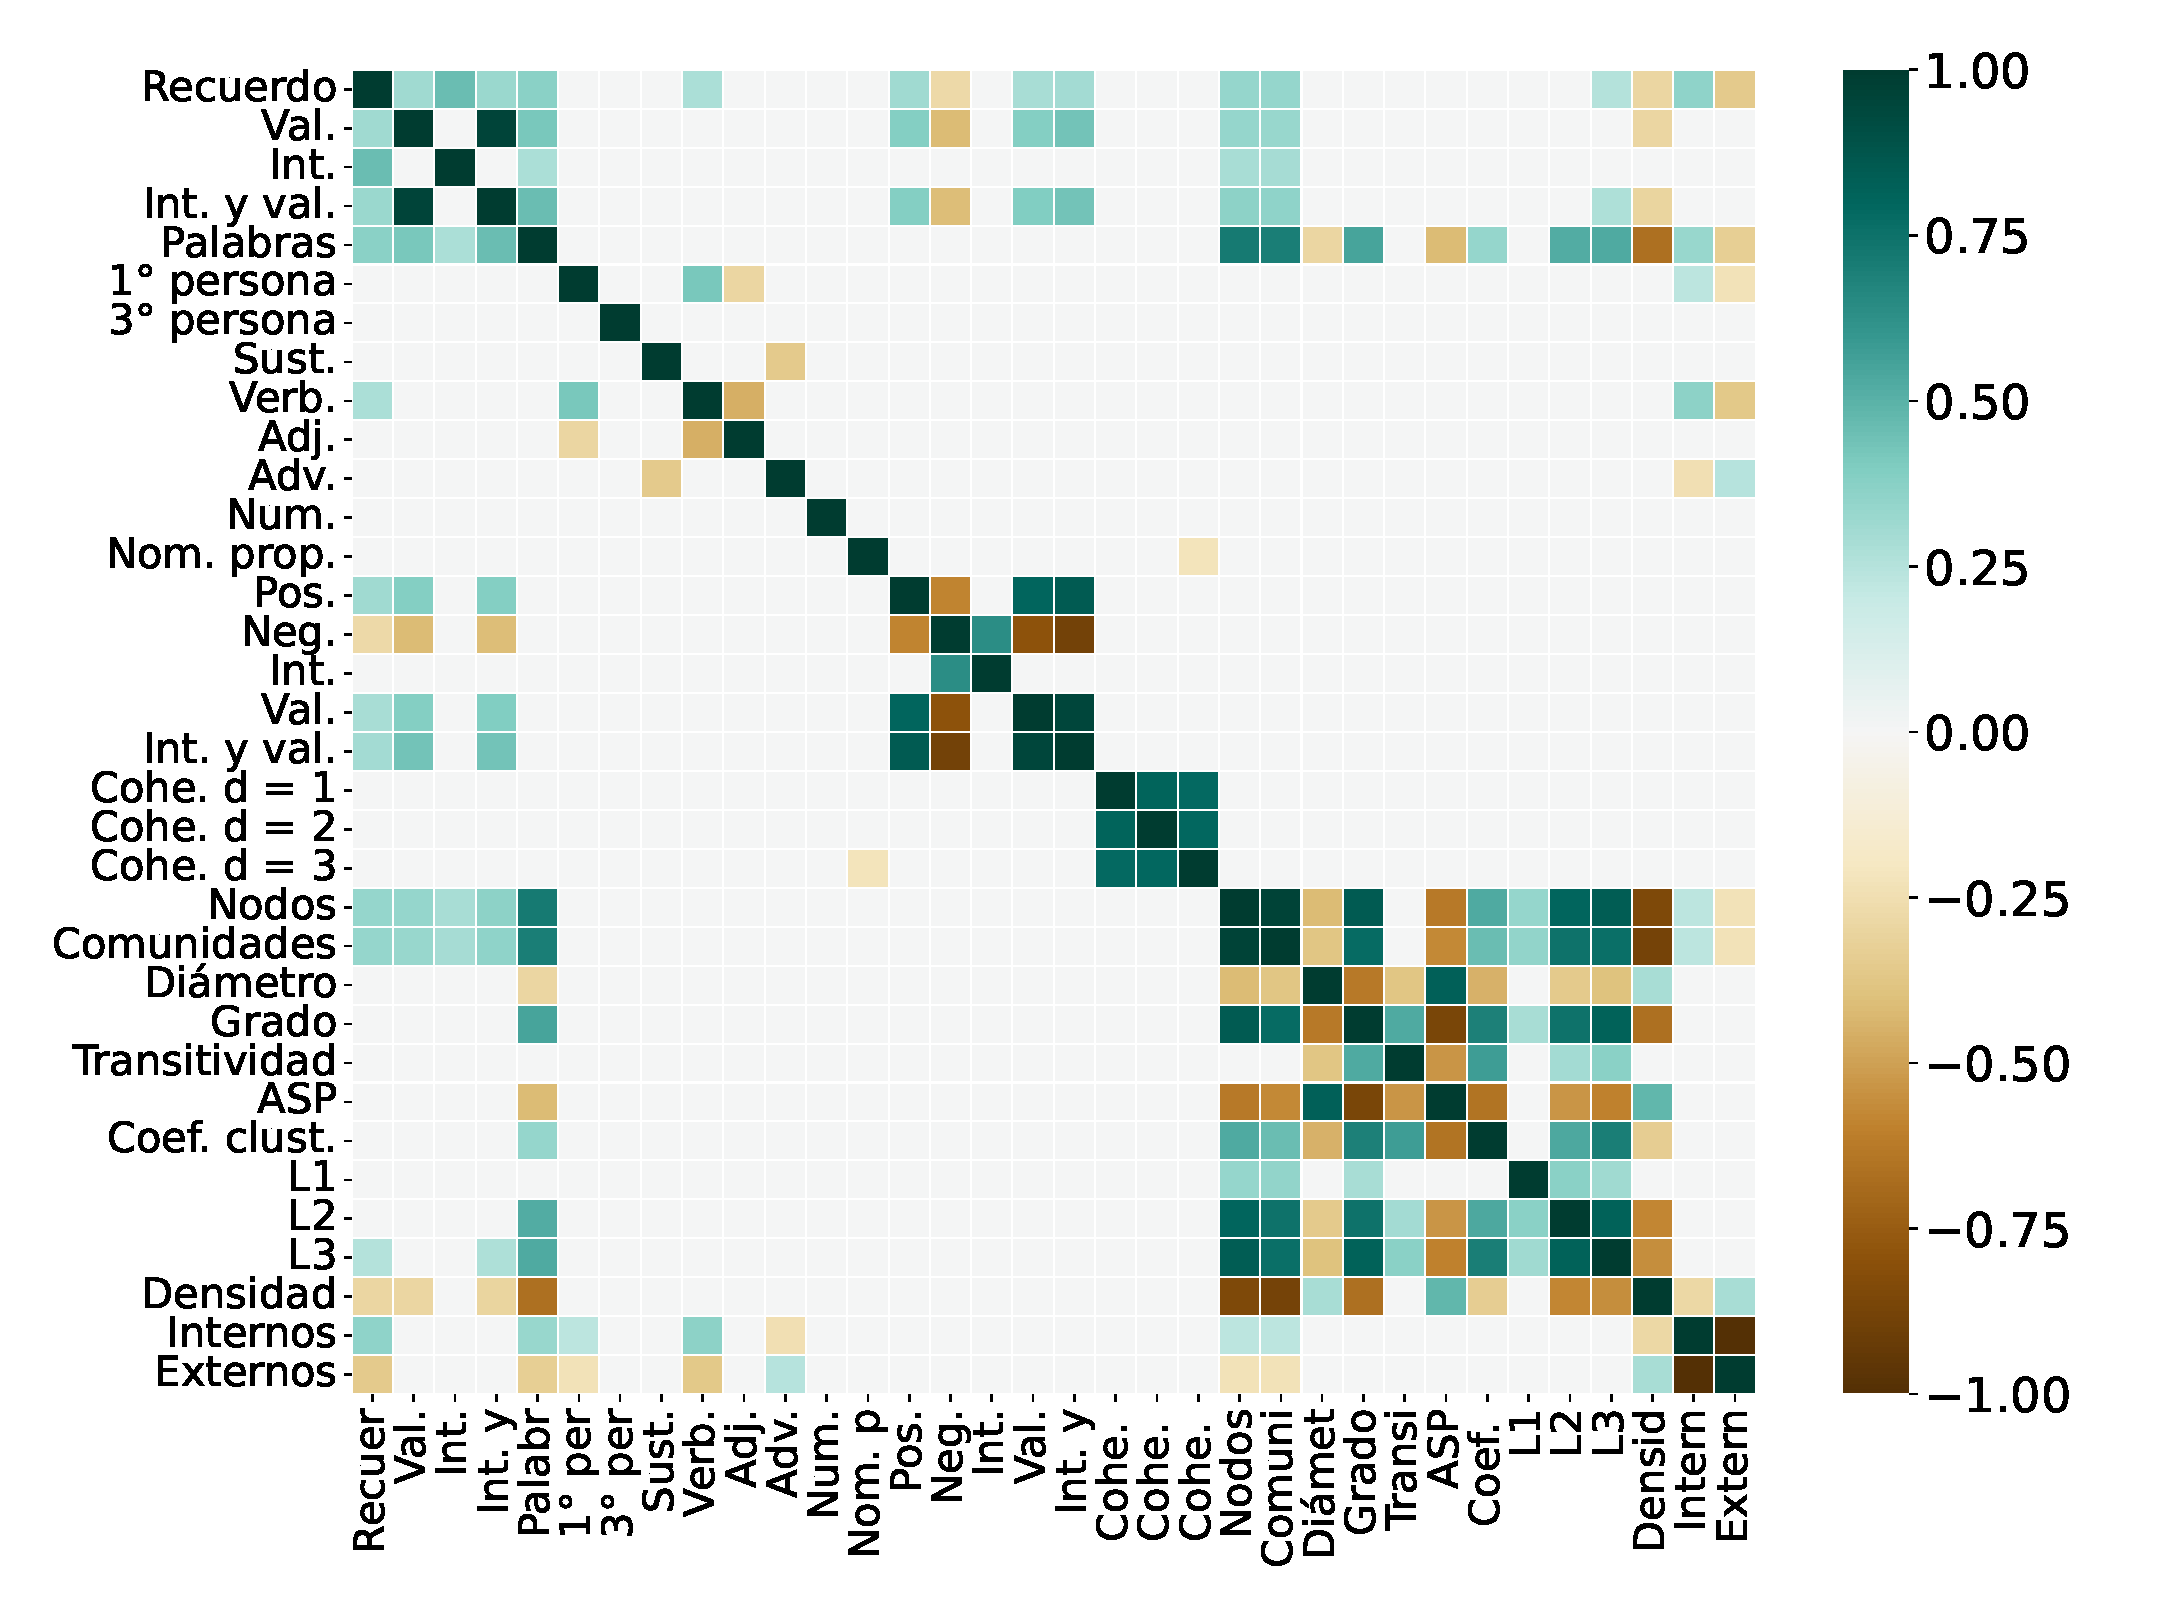
\includegraphics[width = 15cm]{figures/ch03/Correlacion/2correlacion_Segunda.pdf} 
    \caption{Matriz de correlación de los cuantificadores de los relatos y las variables de autopercepción para la segunda entrevista. Solo se presentan en color las correlaciones con un p$_{val}$ menor al significativo (9 $\times$ 10$^{-5}$ = 0,05/número de variables).}
\label{fig:cap3_corrsegt}
\end{figure}

\section{Busqueda de los cuantificadores usando PCA y aprendizaje no supervisado (o clustering)}

En esta sección se utilizará una reducción de dimensionalidad únicamente con las variables obtenidas de los relatos y luego se buscó el agrupamiento natural que surgia de los datos.

El procedimiento fue el siguiente, inicialmente se buscó separar uno de los relatos autobiográficos, el relato de vuelta a la presencialidad del relato de control que era una memoria no consolidada (se le preguntaba a los participantes qué hicieron antes de ir a la entrevista). Se decidió utilizar estos dos relatos pues son los únicos dos que no son memorias colectivas y ponen prioridad a la primera persona. 
Inicialmente se hacía reducción de dimensionalidad y con todas las componentes principales se buscaba el número de grupos óptimo para hacer el agrupamiento con la validación interna dada por Silhuette. Luego se hacía un barrido en el número de componentes principales con las que se buscaría después el agrupamiento con el objetivo de maximizar la validación externa. La validación externa contaba de un test R que compara las etiquetas externas de los relatos con las obtenidas del agrupamiento con clustering. Luego, una vez que se tenía las componentes principales que optimizaban la validación externa se buscaba las variables mas importantes en ellas. Estos resultados se pueden encontrar en la subsección \ref{sec:PCspresvscontrol}.

Solo con las variables mas importantes que se obtenian de las componentes principales que optimizaban la validacióne externa para agrupar los relatos de presencialidad y control se seguía el mismo procedimiento para agrupar los relatos restantes (campeones, CFK y Arabia), lo cual se puede encontrar en la subsección \ref{sec:PCscamparCFK}.

\colorbox{yellow}{pongo esto aca no? Y en métodos solo explico el algoritmo de reducción usado y el de agrupamiento, no esto}

\colorbox{yellow}{en caso de mover esto a métodos, qué escribo aca para introducir?}

\subsection{Memoria autobiográfica contra memoria no consolidada}
\label{sec:PCspresvscontrol}
solo con kmeans mostrar 
primero control vs presencial slihouette para definición de k, mostrar varianza acumulada vs nro PCs, contar que para definir nro PCS se barrió buscando maximizar R (ese gráfico) y PC2 vs PC1 color y forma para cluster y condición, valor de R y matriz de confusión en pie de figura. Mostrar las PCs que usé y hablar de las variables mas importantes de ahí. Mostrar como queda todo en el segundo tiempo usando ESTAS PCs.

\begin{figure}[h]
    \centering
    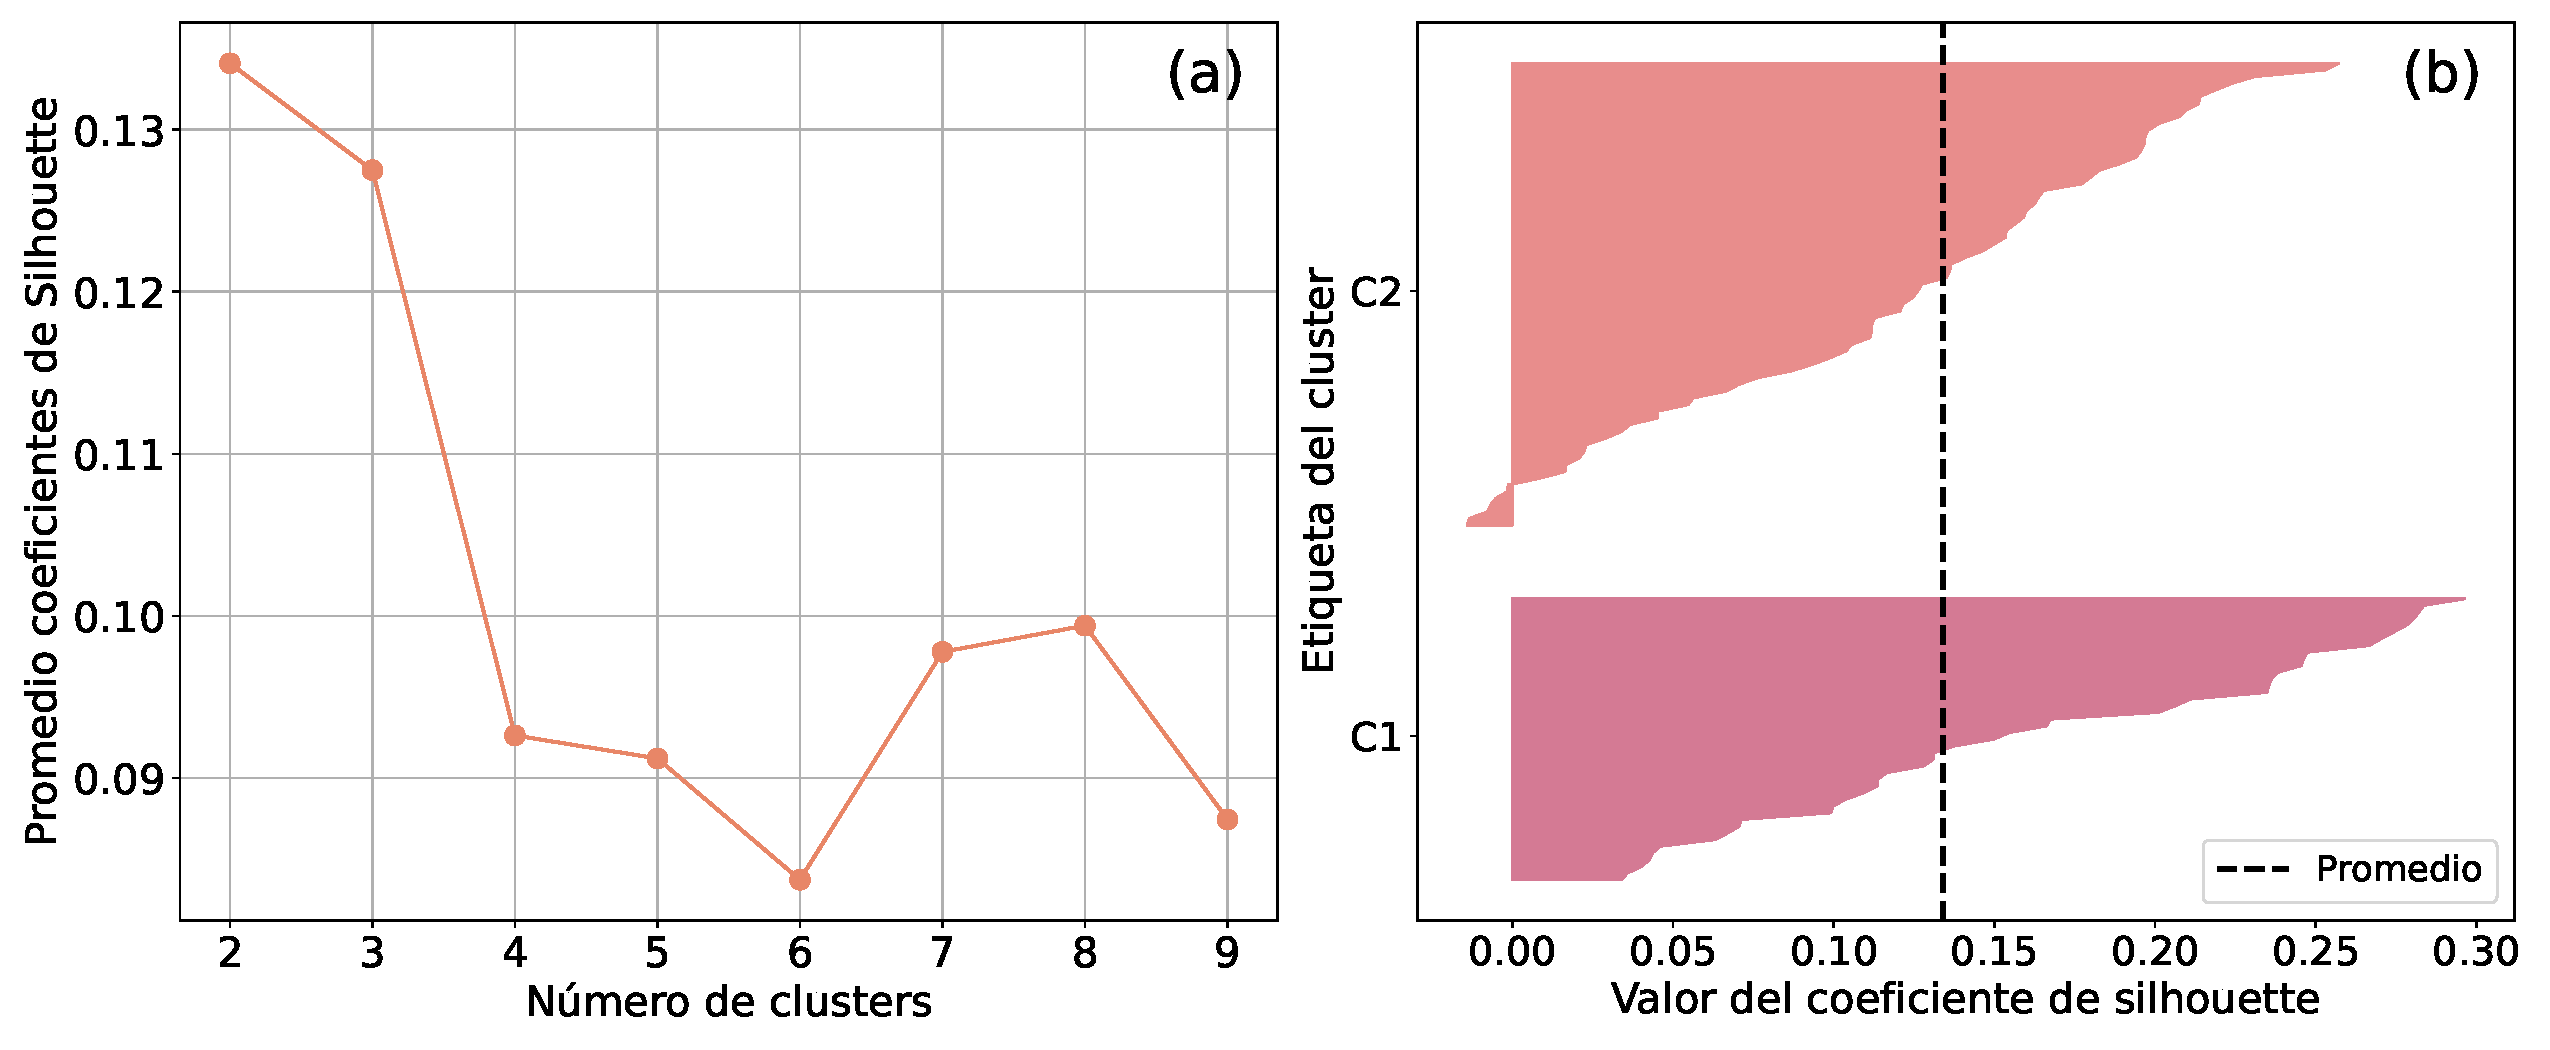
\includegraphics[width = 15cm]{figures/ch03/PCA_clustering/Primer tiempo/silhouette_pres_control.pdf} 
    \caption{Definición de k \textbf{(a)}  \textbf{(b)}}
\label{fig:cap3_defk_controlpres}
\end{figure}

\begin{figure}[h]
    \centering
    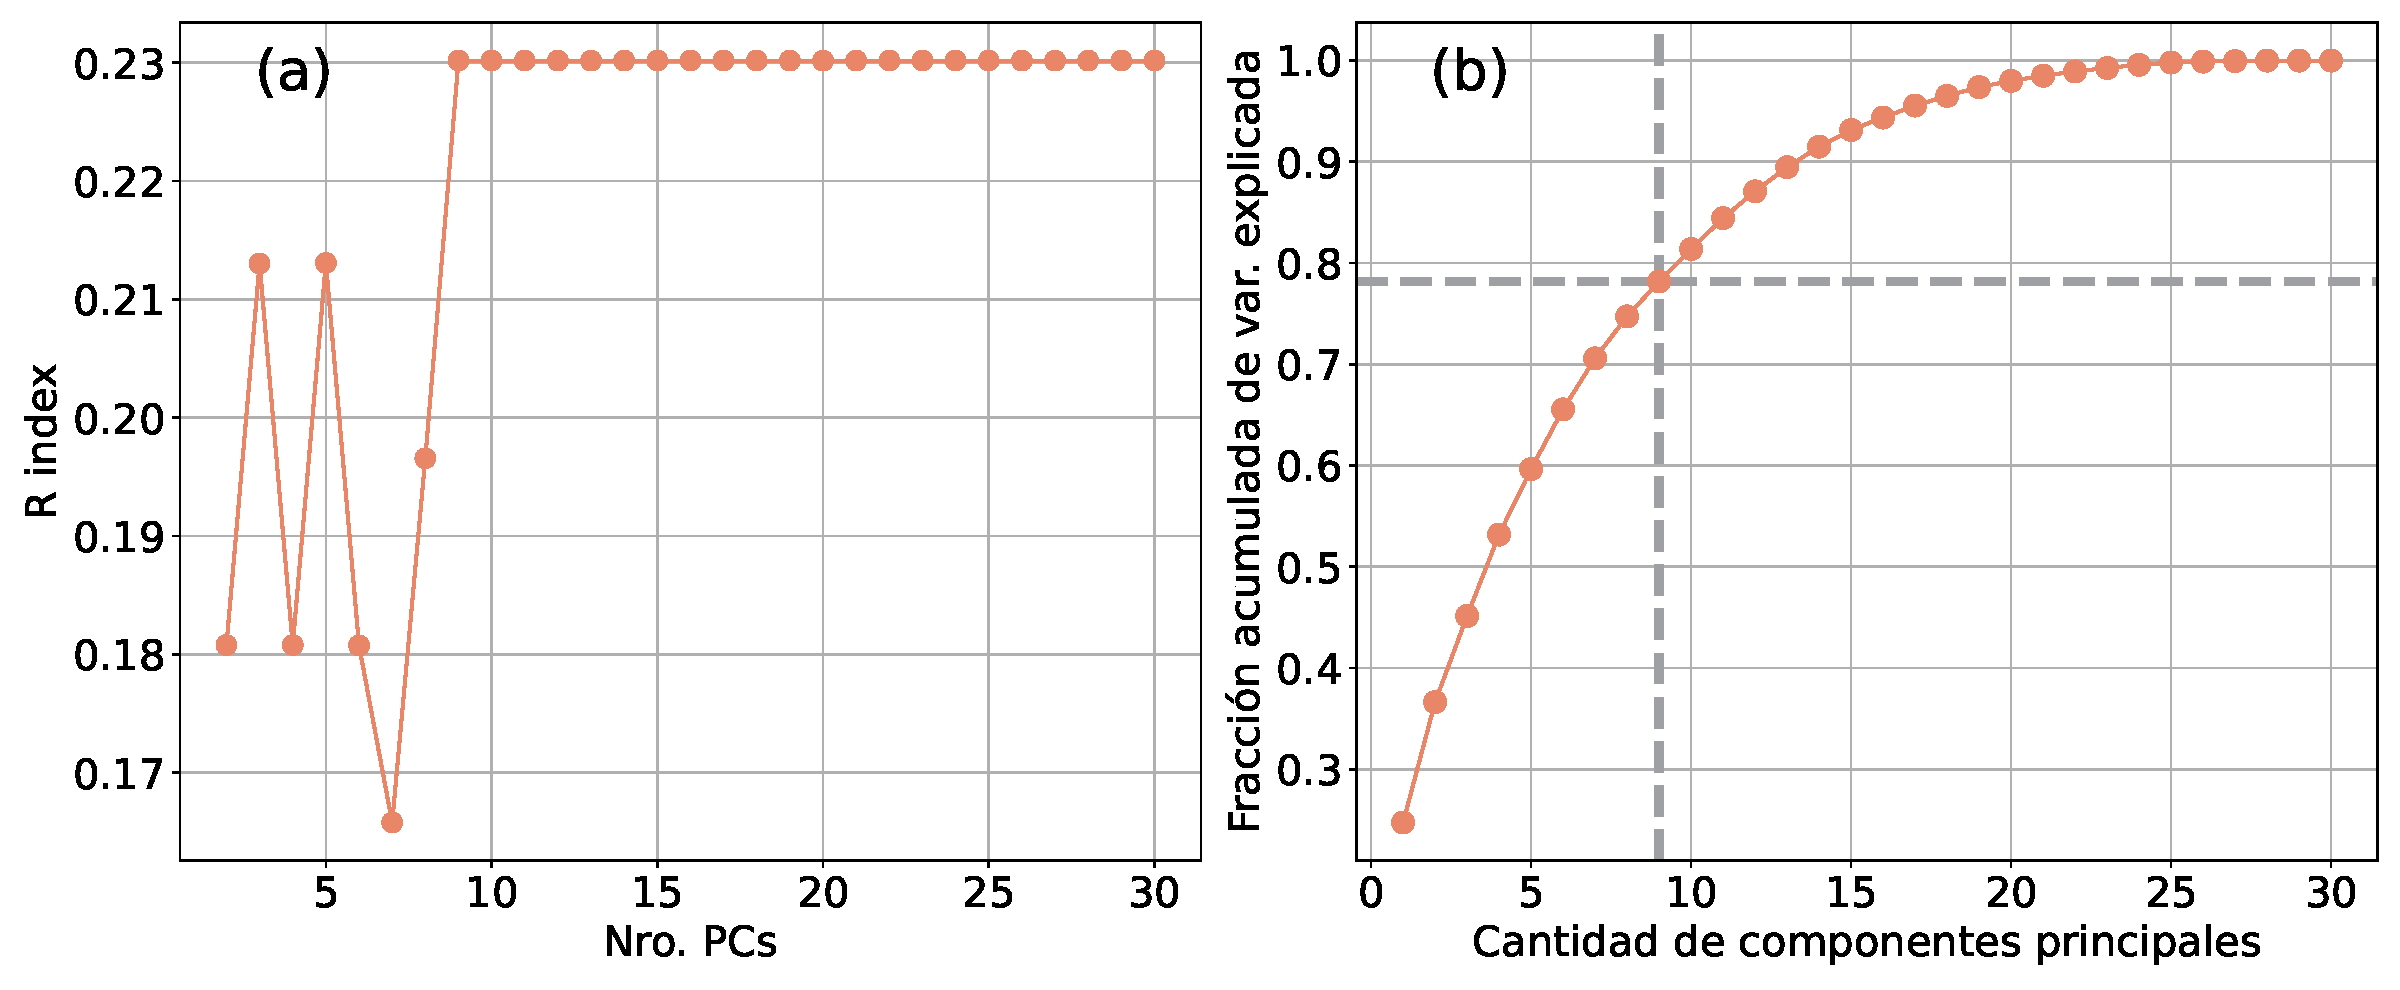
\includegraphics[width = 15cm]{figures/ch03/PCA_clustering/Primer tiempo/RindexyPCs_pres_control.pdf} 
    \caption{Definición número de componentes principales \textbf{(a)}  \textbf{(b)}}
\label{fig:cap3_defpcscontrolpres}
\end{figure}

\begin{figure}[h]
    \centering
    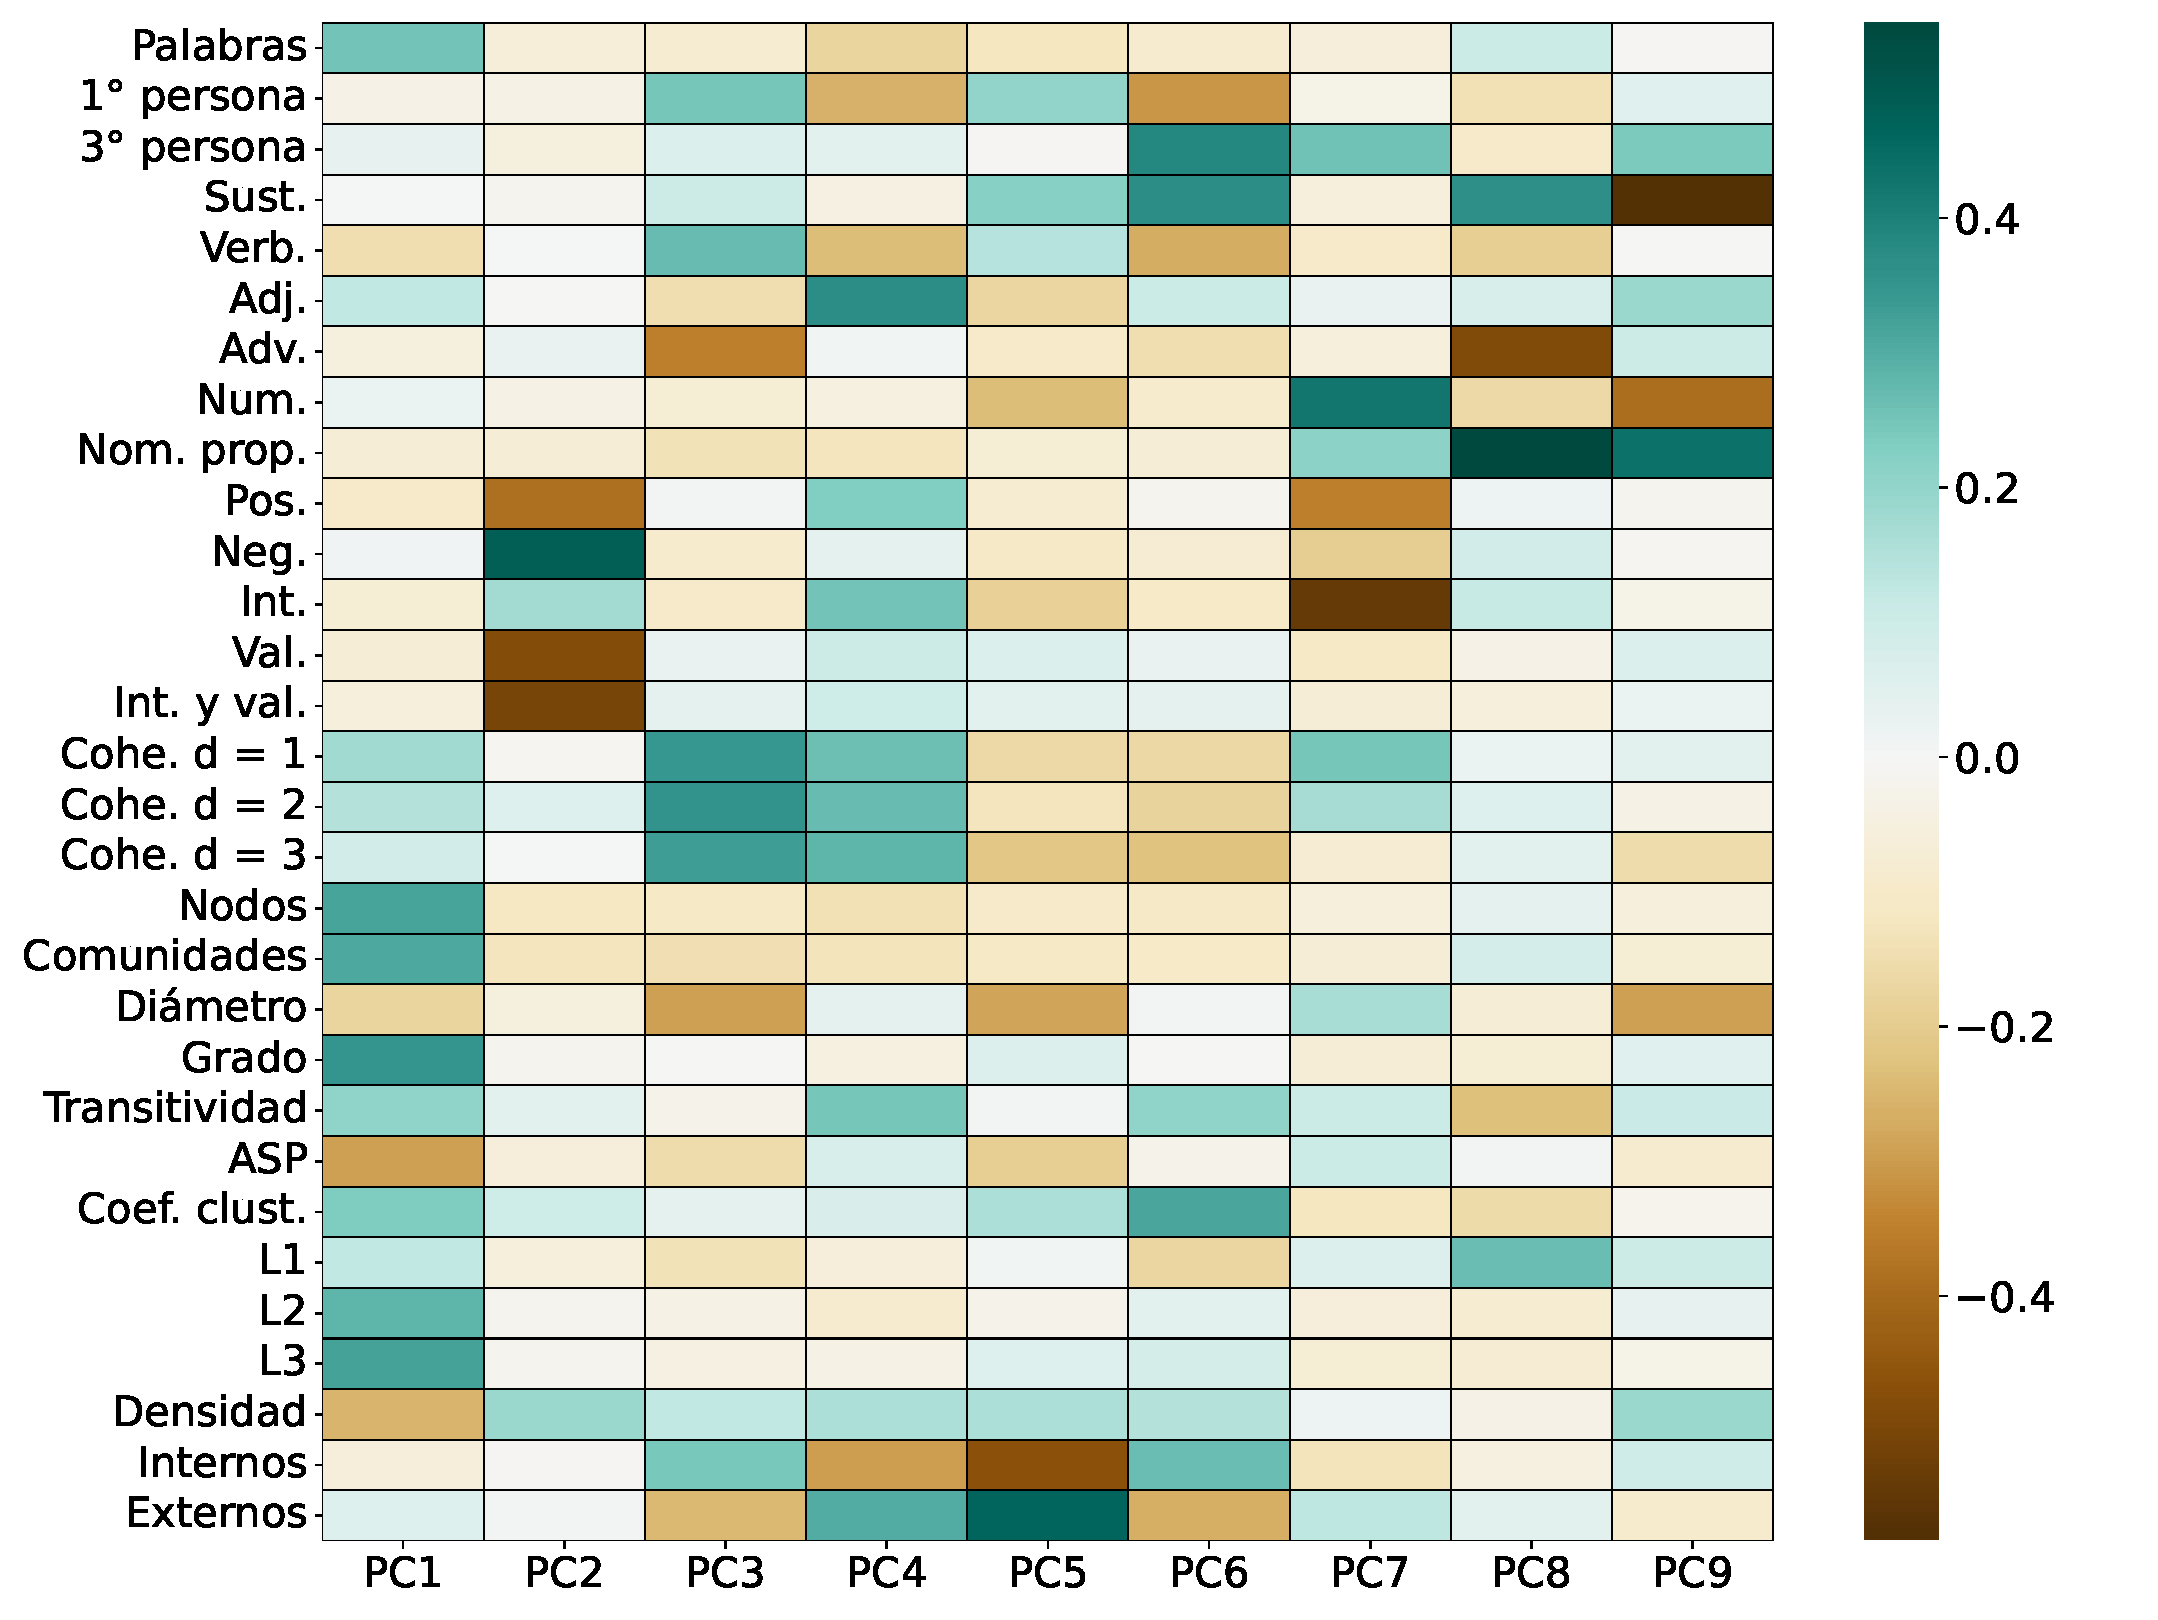
\includegraphics[width = 15cm]{figures/ch03/PCA_clustering/Primer tiempo/9PCs_pres_control.pdf} 
    \caption{Componentes principales de pres y control \textbf{(a)}  \textbf{(b)}}
\label{fig:cap3_9PCscontrolpres}
\end{figure}


\subsection{Memorias con distinta valencia e intensidad}
\label{sec:PCscamparCFK}
Después se busca separar cfk, ar y campeones, primero buscamos usando todas las vars nro pcs vs k silhouette y se definió k, discutir que se ve que aumentar k deja campeones entero pero cfk y arabia quedan juntas, hablar de que son parecidas en emotividad y que se las pasa a considerar un único relato. Dsp  n vs nro pcs una matriz del R para definir n y nro PCs, decir las variables que se eliminan y mostrar varianza acumulada vs nro PCs y dsp las PCs que maximizan R. Mostrar PC1 vs PC2 con los colores y marcadores con condicion y cluster y en pie el R y la matriz de confusión. Mostrar en el segundo tiempo este mismo gráfico.
EN DISCUSIÓN MENCIONÁ QUE A FUTURO SE PODRÍA VER DE AGREGAR COSAS EXTERNAS AL RELATO COMO EL SEM, EL CUESTIONARIO POSTENTREVISTA Y VER SI ESTOS MEJORAN LA PERFORMANCE, PERO QUE HASTA ACA LLEGAMOS CON SOLO LAS VARIABLES DE RELATO QUE USAMOS

\section{Comparación entre ambos tiempos}
Comparamos los ANOVAS de cada condición en el primer tiempo y en el segundo a ver si se ven cambios en los cuantificadores por la edad de la memoria. Hacer gráfico de las PCs con diferencias significativas en el primer tiempo y en el segundo, el gráfico es un histograma de la PC en primero y en segundo a ver para que lado fue y al costado en 2D las vars mas importantes de esta PC boxplots en primero y segundo tiempo (ver carpeta papel el gráfico si no te acordas cual es la idea)

\begin{figure}[h]
    \centering
    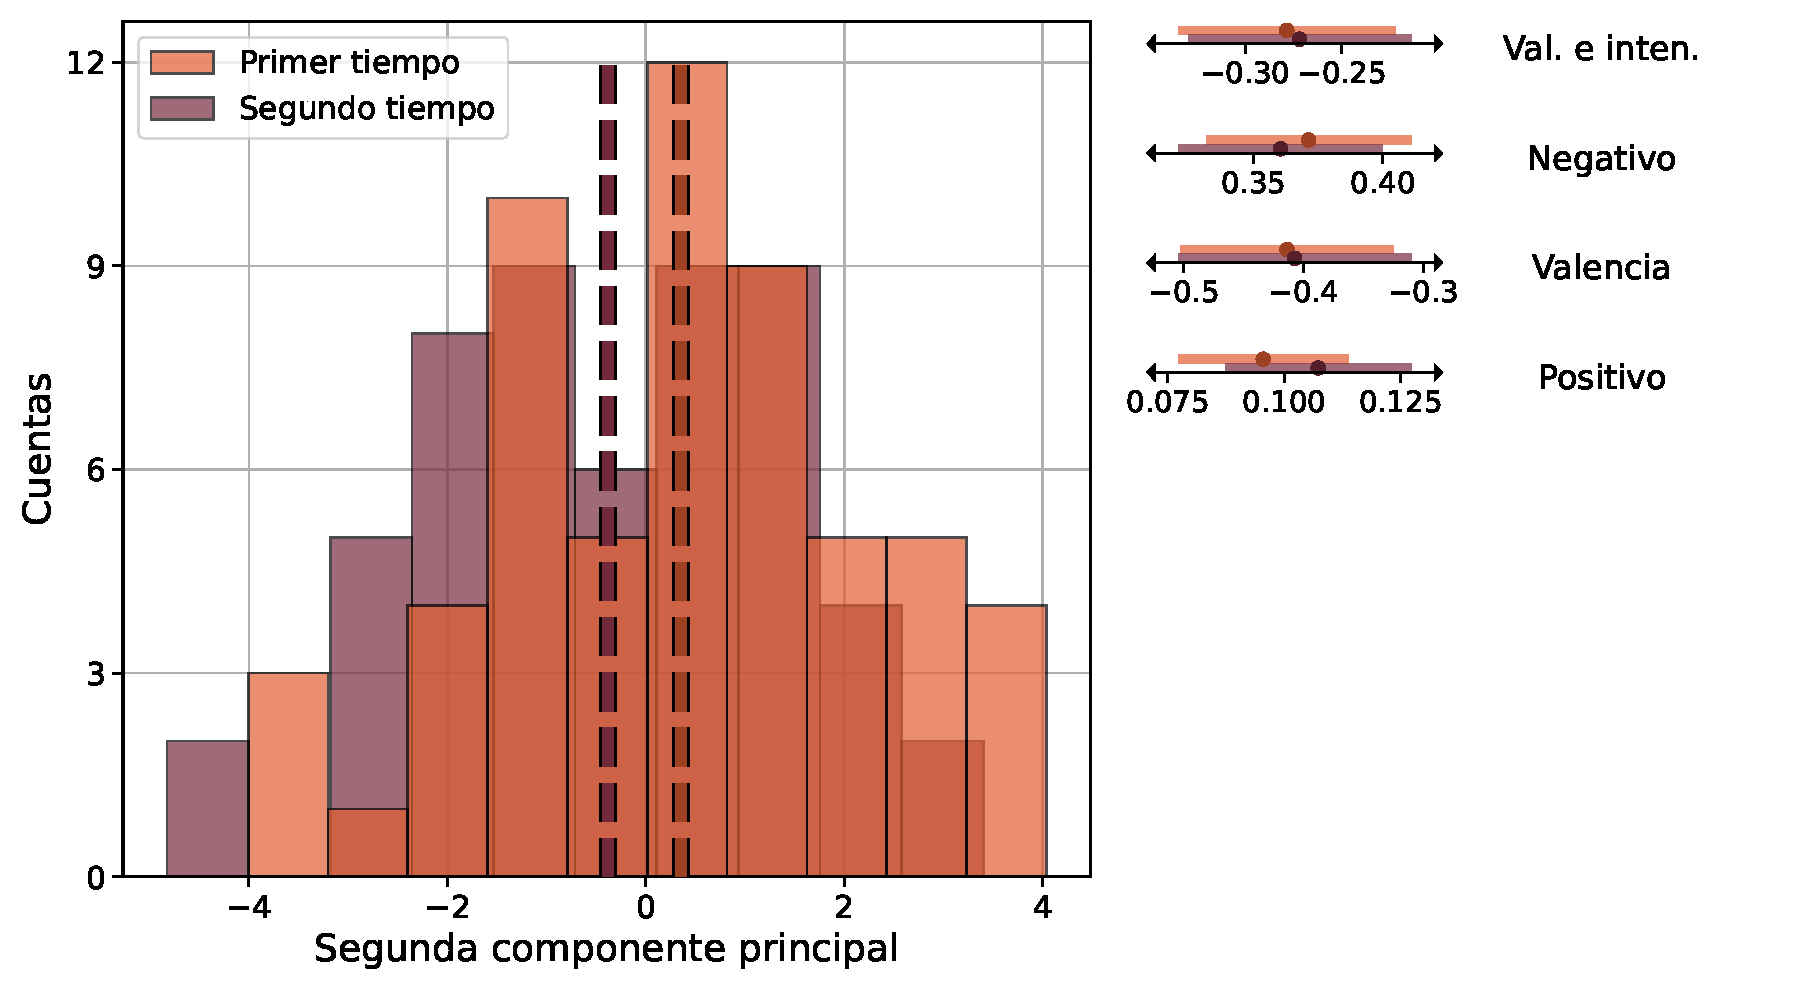
\includegraphics[width = 14cm]{figures/ch03/DosTiempos/arabia_PC2.pdf} 
    \caption{\textbf{(a)}  \textbf{(b)}}
\label{fig:cap3_cysruido_decaimiento_mt}
\end{figure}

